%% abtex2-modelo-trabalho-academico.tex, v-1.9.6 laurocesar
%% Copyright 2012-2016 by abnTeX2 group at http://www.abntex.net.br/ 
%%
%% This work may be distributed and/or modified under the
%% conditions of the LaTeX Project Public License, either version 1.3
%% of this license or (at your option) any later version.
%% The latest version of this license is in
%%   http://www.latex-project.org/lppl.txt
%% and version 1.3 or later is part of all distributions of LaTeX
%% version 2005/12/01 or later.
%%
%% This work has the L PPL maintenance status `maintained'.
%% 
%% The Current Maintainer of this work is the abnTeX2 team, led
%% by Lauro César Araujo. Further information are available on 
%% http://www.abntex.net.br/
%%
%% This work consists of the files abntex2-modelo-trabalho-academico.tex,
%% abntex2-modelo-include-comandos and abntex2-modelo-references.bib
% ------------------------------------------------------------------------
% ------------------------------------------------------------------------
% abnTeX2: Modelo de Trabalho Academico (tese de doutorado, dissertacao de
% mestrado e trabalhos monograficos em geral) em conformidade com 
% ABNT NBR 14724:2011: Informacao e documentacao - Trabalhos academicos -
% Apresentacao
% ------------------------------------------------------------------------
% ------------------------------------------------------------------------
% Personalização para o modelo Udesc 2020 7. ed. revisada e modificada
% MANUAL_2020_09_07_1599489825065_12510.pdf
% Autor: Felipe Joel Zimann (felipezimann@hotmail.com)
% Data: 02/12/2020 v1.0
% Data: 13/02/2021 v1.0.1 alterado tamanho numeração da página para 10pt
% ------------------------------------------------------------------------
% ------------------------------------------------------------------------

\documentclass[
	12pt,					% tamanho da fonte
	openright,				% capítulos começam em pág ímpar (insere página vazia caso preciso)
	oneside,				% para impressão em recto e verso (twoside). Oposto a (oneside)
	a4paper,				% tamanho do papel. 
	chapter=TITLE,			% títulos de capítulos convertidos em letras maiúsculas
	section=TITLE,			% títulos de seções convertidos em letras maiúsculas
	sumario=abnt-6027-2012,
	english,				% idioma adicional para hifenização
	brazil,					% o último idioma é o principal do documento
	fleqn,					% equações alinhadas a esquerda (UDESC/CCT)+
	]{abntex2}

% ----------------------------------------------------------
% Pacotes básicos 
% ----------------------------------------------------------
\usepackage{amsmath}							% Pacote matemático
\usepackage{amssymb}							% Pacote matemático
\usepackage{amsfonts}							% Pacote matemático
%\usepackage{lmodern}							% Usa a fonte Latin Modern		
\usepackage{mathptmx} 							% Usa a fonte Times New Roman	 (UDESC/CCT)
\usepackage[T1]{fontenc}						% Selecao de codigos de fonte.
\usepackage[utf8]{inputenc}						% Codificacao do documento (conversão automática dos acentos)
\usepackage{lastpage}							% Usado pela Ficha catalográfica
\usepackage{indentfirst}						% Indenta o primeiro parágrafo de cada seção.
\usepackage[dvipsnames,table]{xcolor}			% Controle das cores
\usepackage{graphicx}							% Inclusão de gráficos
\usepackage{microtype} 							% para melhorias de justificação
\usepackage{lipsum}								% para geração de dummy text
\usepackage[brazilian,hyperpageref]{backref}	% Paginas com as citações na bibl
\usepackage[alf,abnt-emphasize=bf,abnt-full-initials=yes]{abntex2cite}					% Citações padrão ABNT
%\usepackage[num]{abntex2cite}					% Citações padrão ABNT numérica
\usepackage{adjustbox}							% Pacote de ajuste de boxes
\usepackage{subcaption}							% Inclusão de Subfiguras e sublegendas		
\usepackage{enumitem}							% Personalização de listas
\usepackage{siunitx}							% Grandezas e unidades
\usepackage[section]{placeins}					% Manter as figuras delimitadas na respectiva seção com a opção [section]
\usepackage{multirow}							% Multi colunas nas tabelas
\usepackage{array,tabularx} 					% Pacotes de tabelas
\usepackage{booktabs}							% Pacote de tabela profissonal
\usepackage{rotating}							% Rotacionar figuras e tabelas
\usepackage{xfrac}								% Fazer frações n/d em linha
\usepackage{bm}									% Negrito em modo matemático
\usepackage{xstring}							% Manipulação de strings
\usepackage{pgfplots}							% Pacote de Gráficos
\usepackage{tikz}								% Pacote de Figuras
\usepackage[american, cuteinductors,smartlabels, fulldiode, siunitx, americanvoltages, oldvoltagedirection, smartlabels]{circuitikz}						% Pacote de circuitos elétricos
\usepackage{chemformula}						% Pacote para fórmulas químicas
\usepackage{chngcntr}							% Pacte usado para deixar numeração de equações sequencial (UDESC/CCT)
\counterwithout{equation}{chapter}
% fonte: https://latex.org/forum/viewtopic.php?t=15392

% Comando para deixar numeração das equações contínua (1), (2), (3)... ao invés de organizar por capítulos (1.1)(1.2)... (2.1)(2.2)
%\renewcommand{\theequation}{\arabic{equation}}

%\numberwithin{equation}{section}


% Cabecalho cabeçalho somente com numeração de página 10pt
\makepagestyle{PagNumReduzida}
\makeevenhead{PagNumReduzida}{\ABNTEXfontereduzida\thepage}{}{}
\makeoddhead{PagNumReduzida}{}{}{\ABNTEXfontereduzida\thepage}
%fonte: https://github.com/abntex/abntex2/wiki/HowToCustomizarCabecalhoRodape
%fonte: Manual memoir seção 7.3 pg. 111 pdf http://linorg.usp.br/CTAN/macros/latex/contrib/memoir/memman.pdf 

% Personalização das opções das listas
\setlist[itemize]{leftmargin=\parindent}

% Citação online --- MODIFICAR ---
\newcommand{\citeshort}[1]{\citeauthoronline{#1}~(\citeyear{#1})}

\newcommand{\me}[1]{Elaborado pelo autor (#1).}

% Configuração do pgfplots
\pgfplotsset{compat=newest} %compat=1.14
\pgfplotsset{plot coordinates/math parser=false}
\newlength\figureheight
\newlength\figurewidth

% Libraries do TiKz
\usetikzlibrary{quotes,angles,arrows}
\usetikzlibrary{through,calc,math}
\usetikzlibrary{graphs,backgrounds,fit}
\usetikzlibrary{shapes,positioning,patterns,shadows}
\usetikzlibrary{decorations.pathreplacing}
\usetikzlibrary{shapes.geometric}
\usetikzlibrary{arrows.meta}
\usetikzlibrary{external}

%\tikzexternalize[]
%\tikzexternalenable
%\tikzexternalize
%\tikzexternaldisable
%\tikzset{external/force remake}
%\tikzexternalize[shell escape=-enable-write18]

% Configurações do CircuiTiKz
\ctikzset{bipoles/thickness=1}
%\ctikzset{bipoles/length=1.2cm}
\ctikzset{monopoles/ground/width/.initial=.2}
\ctikzset{bipoles/resistor/height=0.25}
\ctikzset{bipoles/resistor/width=0.6}
\ctikzset{bipoles/capacitor/height=0.5}
\ctikzset{bipoles/capacitor/width=0.15}
\ctikzset{bipoles/generic/height=0.25}
\ctikzset{bipoles/generic/width=0.6}
%\ctikzset{bipoles/capacitor polar/length=0.5}
%\ctikzset{bipoles/diode/height=.375}
%\ctikzset{bipoles/diode/width=.3}
%\ctikzset{tripoles/thyristor/height=.8}
%\ctikzset{tripoles/thyristor/width=1}
\ctikzset{bipoles/vsourcesin/height=.5}
\ctikzset{bipoles/vsourcesin/width=.5}
\ctikzset{bipoles/cvsourceam/height=.6}
\ctikzset{bipoles/cvsourceam/width=.6}
%\ctikzset{tripoles/european controlled voltage source/width=.4}

\tikzstyle{every node}=[font=\footnotesize]
\tikzstyle{every path}=[line width=0.25pt,line cap=round,line join=round]
%\tikzstyle{every path}=[line cap=round,line join=round]


% Definição de cores MATLAB
\definecolor{matlab_blue}{rgb}	{         0,    0.4470,    0.7410}
\definecolor{matlab_orange}{rgb}{    0.8500,    0.3250,    0.0980}
\definecolor{matlab_yellow}{rgb}{    0.9290,    0.6940,    0.1250}
\definecolor{matlab_violet}{rgb}{    0.4940,    0.1840,    0.5560}
\definecolor{matlab_green}{rgb}	{	 0.4660,    0.6740,    0.1880}
\definecolor{matlab_lblue}{rgb}	{    0.3010,    0.7450,    0.9330}
\definecolor{matlab_red}{rgb}	{    0.6350,    0.0780,    0.1840}

% Personalização das legendas
\usepackage[format = plain, %hang
	justification = centering,
	labelsep = endash,
	singlelinecheck = false,
	skip = 6pt,
	listformat = simple]{caption}

% Personalização das unidades
\sisetup{output-decimal-marker = {,}}
\sisetup{exponent-product = \cdot, output-product = \cdot}
\sisetup{tight-spacing=true}
\sisetup{group-digits = false}

% Personalizações de tipo de colunas de tabelas
\newcolumntype{L}[1]{>{\raggedright\let\newline\\\arraybackslash\hspace{0pt}}m{#1}}
\newcolumntype{C}[1]{>{\centering\let\newline\\\arraybackslash\hspace{0pt}}m{#1}}
\newcolumntype{R}[1]{>{\raggedleft\let\newline\\\arraybackslash\hspace{0pt}}m{#1}}

% Personalizações de cores da UDESC
\definecolor{CapaAmareloUDESC}{RGB}{243,186,83}		% Especializacao
\definecolor{CapaVerdeUDESC}{RGB}{0,112,52}			% Mestrado
\definecolor{CapaVermelhoUDESC}{RGB}{171,35,21}		% Doutorado
\definecolor{CapaAzulUDESC}{RGB}{38,54,118} 		% Pós-Doutorado

% CONFIGURAÇÕES DE PACOTES
% Configurações do pacote backref
% Usado sem a opção hyperpageref de backref
\renewcommand{\backrefpagesname}{Citado na(s) página(s):~}
% Texto padrão antes do número das páginas
\renewcommand{\backref}{}
% Define os textos da citação
\renewcommand*{\backrefalt}[4]{
	\ifcase #1 %
		Nenhuma citação no texto.%
	\or
		Citado na página #2.%
	\else
		Citado #1 vezes nas páginas #2.%
	\fi}%

% alterando o aspecto da cor azul
%\definecolor{blue}{RGB}{41,5,195}

% informações do PDF
\makeatletter
\hypersetup{
	%pagebackref=true,
	pdftitle={\@title},
	pdfauthor={\@author},
	pdfsubject={\imprimirpreambulo},
	pdfcreator={LaTeX with abnTeX2},
	pdfkeywords={abnt}{latex}{abntex}{abntex2}{trabalho academico},
	colorlinks=true,       		% false: boxed links; true: colored links
	linkcolor=black,          	% color of internal links
	citecolor=black,        	% color of links to bibliography
	filecolor=black,      		% color of file links
	urlcolor=black,
	bookmarksdepth=4
}
\makeatother


\makeatletter
\newcommand{\includetikz}[1]{%
	\tikzsetnextfilename{#1}%
	\input{#1.tex}%
}
\makeatother

% ---
% Possibilita criação de Quadros e Lista de quadros.
% Ver https://github.com/abntex/abntex2/issues/176
%
\newcommand{\quadroname}{Quadro}
\newcommand{\listofquadrosname}{Lista de quadros}

\newfloat[chapter]{quadro}{loq}{\quadroname}
\newlistof{listofquadros}{loq}{\listofquadrosname}
\newlistentry{quadro}{loq}{0}

% configurações para atender às regras da ABNT
\setfloatadjustment{quadro}{\centering}
\counterwithout{quadro}{chapter}
\renewcommand{\cftquadroname}{\quadroname\space}
\renewcommand*{\cftquadroaftersnum}{\hfill--\hfill}

\setfloatlocations{quadro}{hbtp} % Ver https://github.com/abntex/abntex2/issues/176
% ---


% Espaçamento depois do título
\setlength{\afterchapskip}{0.7\baselineskip}
% O tamanho do parágrafo é dado por:
\setlength{\parindent}{1.25cm}
% Controle do espaçamento entre um parágrafo e outro:
\setlength{\parskip}{0.0cm}  % tente também \onelineskip
%\SingleSpacing % Espaçamento simples 
\OnehalfSpacing % Espaçamento 1,5 (UDESC/CCT)
%\DoubleSpacing	% Espaçamento duplo

% ---
% Margens - NBR 14724/2011 - 5.1 Formato
% ---
\setlrmarginsandblock{3cm}{2cm}{*}
\setulmarginsandblock{3cm}{2cm}{*}
\checkandfixthelayout[fixed]
% ---


% To use externalize consider
%https://tex.stackexchange.com/questions/182783/tikzexternalize-not-compatible-with-miktex-2-9-abntex2-package
%Lauro Cesar digged into the problem until he came with a solution for me to test. And it Works!
%
%According to this link:
%
%The package calc changed the commands \setcounter and friends to be fragile. So you have to make them robust. The example below uses etoolbox with \robustify:
%
\usepackage{etoolbox}
\robustify\setcounter
\robustify\addtocounter
\robustify\setlength
\robustify\addtolength


%% How to silence memoir class warning against the use of caption package?
%% https://tex.stackexchange.com/questions/391993/how-to-silence-memoir-class-warning-against-the-use-of-caption-package
%\usepackage{silence}
%\WarningFilter*{memoir}{You are using the caption package with the memoir class}
%\WarningFilter*{Class memoir Warning}{You are using the caption package with the memoir class}

% --------------------------------------------------------
% INICIO DAS CUSTOMIZACOES PARA A UDESC
% --------------------------------------------------------

% --------------------------------------------------------
% Fontes padroes de part, chapter, section, subsection e subsubsection
% --------------------------------------------------------
% --- Chapter ---
\renewcommand{\ABNTEXchapterfont}{\fontseries{b}} %\bfseries
\renewcommand{\ABNTEXchapterfontsize}{\normalsize}
% --- Part ---
\renewcommand{\ABNTEXpartfont}{\ABNTEXchapterfont}
\renewcommand{\ABNTEXpartfontsize}{\LARGE}
% --- Section ---
\renewcommand{\ABNTEXsectionfont}{\normalfont}
\renewcommand{\ABNTEXsectionfontsize}{\normalsize}
% --- SubSection ---
\renewcommand{\ABNTEXsubsectionfont}{\fontseries{b}} %\bfseries
\renewcommand{\ABNTEXsubsectionfontsize}{\normalsize}
% --- SubSubSection ---
\renewcommand{\ABNTEXsubsubsectionfont}{\itshape}
\renewcommand{\ABNTEXsubsubsectionfontsize}{\normalsize}

\renewcommand{\ABNTEXsubsubsubsectionfont}{\normalfont}
\renewcommand{\ABNTEXsubsubsubsectionfontsize}{\normalsize}
% ---

% --------------------------------------------------------
% Fontes das entradas do sumario
% --------------------------------------------------------

\renewcommand{\cftpartfont}{\ABNTEXpartfont\selectfont}
\renewcommand{\cftpartpagefont}{\normalsize\selectfont}

\renewcommand{\cftchapterfont}{\ABNTEXchapterfont\selectfont}
\renewcommand{\cftchapterpagefont}{\normalsize\selectfont}

\renewcommand{\cftsectionfont}{\ABNTEXsectionfont\selectfont}
\renewcommand{\cftsectionpagefont}{\normalsize\selectfont}

\renewcommand{\cftsubsectionfont}{\ABNTEXsubsectionfont\selectfont}
\renewcommand{\cftsubsectionpagefont}{\normalsize\selectfont}

\renewcommand{\cftsubsubsectionfont}{\normalfont\itshape\selectfont}
\renewcommand{\cftsubsubsectionpagefont}{\normalsize\selectfont}

\renewcommand{\cftparagraphfont}{\normalfont\selectfont}
\renewcommand{\cftparagraphpagefont}{\normalsize\selectfont}

% --------------------------------------------------------
% Usando os pacotes hyperref, uppercase... 
% Para deixar a section do toc uppercase precisa de:
% --------------------------------------------------------
\usepackage{textcase}

\makeatletter

\let\oldcontentsline\contentsline
\def\contentsline#1#2{%
\expandafter\ifx\csname l@#1\endcsname\l@section
	\expandafter\@firstoftwo
\else
	\expandafter\@secondoftwo
\fi
{%
\oldcontentsline{#1}{\MakeTextUppercase{#2}}%
}{%
\oldcontentsline{#1}{#2}%
}%
}
\makeatother

% --------------------------------------------------------
% Renomenando as entradas de APÊNDICES E ANEXOS
% --------------------------------------------------------

\renewcommand{\apendicesname}{AP\^ENDICES}
\renewcommand{\anexosname}{ANEXOS}


% Manipulação de Strings
%\RequirePackage{xstring}

% Comando para inverter sobrenome e nome
\newcommand{\invertname}[1]{%
	\StrBehind{#1}{{}}, \StrBefore{#1}{{}}%
}%


% --------------------------------------------------------
% Alterando os estilos de Caption e Fonte
% --------------------------------------------------------
\makeatletter
% Define o comando \fonte que respeita as configurações de caption do memoir ou do caption
\renewcommand{\fonte}[2][\fontename]{%
	\M@gettitle{#2}%
	\memlegendinfo{#2}%
	\par
	\begingroup
	\@parboxrestore
	\if@minipage
		\@setminipage
	\fi
	\ABNTEXfontereduzida
	\configureseparator
	\captiondelim{\ABNTEXcaptionfontedelim}
	\@makecaption{#1}{\ignorespaces #2}\par
	\endgroup}


\captionstyle[\raggedright]{\raggedright}

\makeatother

\setlength{\cftbeforechapterskip}{0pt plus 0pt}
\renewcommand*{\insertchapterspace}{}

\newlength{\mylen}	% New length to use with spacing
\setlength{\mylen}{1pt}

\setlength{\cftbeforechapterskip}{\mylen}
\setlength{\cftbeforesectionskip}{\mylen}
\setlength{\cftbeforesubsectionskip}{\mylen}
\setlength{\cftbeforesubsubsectionskip}{\mylen}
\setlength{\cftbeforesubsubsubsectionskip}{\mylen}


% ---
% Ajuste das listas de abreviaturas e siglas ; e símbolos [Personalizada para UDESC com espaçamento 1,5]
% ---

% ---
% Redefinição da Lista de abreviaturas e siglas [Personalizada para UDESC com espaçamento 1,5]
\renewenvironment{siglas}{%
	\pretextualchapter{\listadesiglasname}
	\begin{symbols}
		\setlength{\itemsep}{0pt}	% Ajuste para Espaçamento 1,5 (UDESC/CCT)
		}{% 
	\end{symbols}
	\cleardoublepage
}
% ---

% ---
% Redefinição da Lista de símbolos [Personalizada para UDESC com espaçamento 1,5]
\renewenvironment{simbolos}{%
	\pretextualchapter{\listadesimbolosname}
	\begin{symbols}
		\setlength{\itemsep}{0pt}	% Ajuste para Espaçamento 1,5 (UDESC/CCT)
		}{%
	\end{symbols}
	\cleardoublepage
}
% ---





% ---
% FIM DAS CUSTOMIZACOES PARA A  Universidade do Estado de Santa Catarina - UDESC/CCT
% ---





	% Incliu pacotes básicos 

% -----------------------------------------------------------------
% Você pode adicionar seus pacotes a partir desta linha;
% -----------------------------------------------------------------

%\usepackage[showframe,pass]{geometry}
%\usepackage[11,12]{pagesel}

% -----------------------------------------------------------------
% Informações de dados para CAPA e FOLHA DE ROSTO
% -----------------------------------------------------------------
\titulo{FinTrackr}%

\autor{Dênis Diego {}Marx \and Thiago Artur {}Schumann}%
\orientador{Mattheus da Hora {}Franca}%
%\coorientador{Nome do coorientador{} Sobrenome}%

% ATENÇÃO: O símbolo {} indica o sobrenome para a ficha catalográfica.
% Exemplo: Sherlock Holmes {}da Silva para sobrenomes compostos;
% Exemplo: Arnold Alois {}Schwarzenegger para sobrenome simples.

\instituicao{Universidade do Estado de Santa Catarina, Centro de Educação Superior do Alto Vale do Itajaí, Departamento de Engenharia de Software}%

%\tipotrabalho{Tese (Doutorado)}
\tipotrabalho{Trabalho acadêmico (Graduação)}

%\preambulo{Tese apresentada ao Programa de Pós--Graduação em Engenharia Elétrica do Centro de Ciências Tecnológicas da Universidade do Estado de Santa Catarina, como requisito parcial para a obtenção do grau de Doutor em Engenharia Elétrica.}

\preambulo{Dissertação apresentada ao Programa de Pós--Graduação em Engenharia Elétrica do Centro de Ciências Tecnológicas da Universidade do Estado de Santa Catarina, como requisito parcial para a obtenção do grau de Mestre em Engenharia Elétrica.}

\local{Ibirama}%

\data{\the\year}%
% ---

% compila o indice
\makeindex

% -----------------------------------------------------------------
% Início do documento
% -----------------------------------------------------------------
\begin{document}

\selectlanguage{brazil}
\frenchspacing  % Retira espaço extra obsoleto entre as frases.

% -----------------------------------------------------------------
% ELEMENTOS PRÉ-TEXTUAIS
% -----------------------------------------------------------------
\pretextual

% Você pode comentar os elementos que não deseja em seu trabalho;

% A capa pode ser escolhida dentro do arquivo Capa.tex (TCC, Master, Doc, ...)
% ---
% Capa
% ---


% --------------------------------------------------------
% Capa Padrão
% --------------------------------------------------------
\renewcommand{\imprimircapa}{%
	\begin{capa}%
		\center

		{\fontseries{b}\selectfont\MakeTextUppercase{UNIVERSIDADE DO ESTADO DE SANTA CATARINA -- UDESC}}

		{\fontseries{b}\selectfont\MakeTextUppercase{CENTRO DE EDUCAÇÃO SUPERIOR DO ALTO VALE DO ITAJAÍ -- CEAVI  }}

		{\fontseries{b}\selectfont\MakeTextUppercase{ENGENHARIA DE SOFTWARE -- ESO  }}

		\vfill

		{\fontseries{b}\selectfont\MakeTextUppercase{\normalsize\imprimirautor}}

		\vfill
		\begin{center}
			{\fontseries{b}\selectfont\MakeTextUppercase{\imprimirtitulo}}
		\end{center}
		\vfill

		\vfill

		{\fontseries{b}\selectfont\MakeTextUppercase{\imprimirlocal}}
		\par
		{\fontseries{b}\selectfont \imprimirdata}
		\vspace*{1cm}
	\end{capa}
}



\imprimircapa				% Capa padrão

					% Elemento Obrigatório
%% ---
% Folha de rosto
% ---








% --------------------------------------------------------
% folha de rosto 
% --------------------------------------------------------

\makeatletter

\renewcommand{\folhaderostocontent}{
	\begin{center}
		
		{\fontseries{b}\selectfont\MakeTextUppercase{\imprimirautor}}
		
		\vfill
		
		\begin{center}
			{\fontseries{b}\selectfont\MakeTextUppercase{\imprimirtitulo}}
		\end{center}
	
		\vspace*{1.5cm}

		\abntex@ifnotempty{\imprimirpreambulo}{%
			\hspace{.45\textwidth}
			{\begin{minipage}{.5\textwidth}
					\SingleSpacing
					\imprimirpreambulo\par
					\vspace*{4pt}
					{\imprimirorientadorRotulo~\imprimirorientador\par}
					\abntex@ifnotempty{\imprimircoorientador}{%
						{\imprimircoorientadorRotulo~\imprimircoorientador}%
					}%
			\end{minipage}}%
		}%
	
		
		\vfill
		
	{\fontseries{b}\selectfont\MakeTextUppercase{\imprimirlocal}}
	\par
	{\fontseries{b}\selectfont \imprimirdata}
	\vspace*{1cm}
	\end{center}
}


% (o * indica que haverá a ficha bibliográfica)
% ---
\imprimirfolhaderosto*
% ---


			% Elemento Obrigatório
% Caso não utilize a Ficha Catalográfica entre na folha de rosto e retire o * de dentro do arquivo FolhadeRosto
%
% ---
% Inserir a ficha bibliografica
% ---

% Isto é um exemplo de Ficha Catalográfica, ou ``Dados internacionais de
% catalogação-na-publicação''. Você pode utilizar este modelo como referência. 
% Porém, provavelmente a biblioteca da sua universidade lhe fornecerá um PDF
% com a ficha catalográfica definitiva após a defesa do trabalho. Quando estiver
% com o documento, salve-o como PDF no diretório do seu projeto e substitua todo
% o conteúdo de implementação deste arquivo pelo comando abaixo:



% \begin{fichacatalografica}
%     \includepdf{fig_ficha_catalografica.pdf}
% \end{fichacatalografica}


%	\setlength{\parindent}{0cm}
%	\setlength{\parskip}{0pt}
\begin{fichacatalografica}
	%\sffamily
	%\rmfamily
	\ttfamily \hbadness=10000
	\vspace*{\fill}					% Posição vertical
	\begin{center}					% Minipage Centralizado
		Para gerar a ficha catalográfica de teses e \\
		dissertações acessar o link:  \\
		https://www.udesc.br/bu/manuais/ficha

		\vspace*{8pt}

		%	\begin{minipage}[c]{8cm}
		%	\centering \sffamily
		%	 Ficha catalográfica elaborada pelo(a) autor(a), com auxílio do programa de geração automática da Biblioteca Setorial do CCT/UDESC
		%	\end{minipage}
		\fbox{\begin{minipage}[c]{12.5cm}		% Largura
				\flushright
				{\begin{minipage}[c]{10.5cm}		% Largura
						\vspace{1.25cm}
						%\footnotesize
						\setlength{\parindent}{1.5em}
						\noindent \invertname{\imprimirautor} \par
						\imprimirtitulo{ }/{ }\imprimirautor. -- \imprimirlocal, \imprimirdata .\par
						\pageref{LastPage} p. : il. ; 30 cm.\par
						\vspace{1.5em}
						\imprimirorientadorRotulo~\imprimirorientador.\par
						\imprimircoorientadorRotulo~\imprimircoorientador.\par
						\imprimirtipotrabalho~--~\imprimirinstituicao, \imprimirlocal, \imprimirdata.\par
						\vspace{1.5em}
						1. Palavra-chave.
						2. Palavra-chave.
						3. Palavra-chave.
						4. Palavra-chave.
						5. Palavra-chave.
						I. \invertname{\imprimirorientador}.
						II. \invertname{\imprimircoorientador}.
						III. \imprimirinstituicao.
						IV. Título. %
						\vspace{1.25cm}	%		
					\end{minipage}%
				}% 
			\end{minipage}}%

		\vspace*{0.5cm}

	\end{center}
\end{fichacatalografica}


%\begin{fichacatalografica}
%	\sffamily
%	\vspace*{\fill}					% Posição vertical
%	\begin{center}					% Minipage Centralizado
%	\fbox{\begin{minipage}[c][8cm]{13.5cm}		% Largura
%	\small
%	\imprimirautor
%	%Sobrenome, Nome do autor
%	
%	\hspace{0.5cm} \imprimirtitulo  / \imprimirautor. --
%	\imprimirlocal, \imprimirdata-
%	
%	\hspace{0.5cm} \pageref{LastPage} p. : il. (algumas color.) ; 30 cm.\\
%	
%	\hspace{0.5cm} \imprimirorientadorRotulo~\imprimirorientador\\
%	
%	\hspace{0.5cm}
%	\parbox[t]{\textwidth}{\imprimirtipotrabalho~--~\imprimirinstituicao,
%	\imprimirdata.}\\
%	
%	\hspace{0.5cm}
%		1. Palavra-chave1.
%		2. Palavra-chave2.
%		3. Palavra-chave3.
% 		4. Palavra-chave4.
%		5. Palavra-chave5.
%		I. Orientador.
%		II. Universidade xxx.
%		III. Faculdade de xxx.
%		IV. Título 			
%	\end{minipage}}
%	\end{center}
%\end{fichacatalografica}
% ---

	% Elemento Obrigatório (Verso da Folha)
%
% ---
% Inserir errata
% ---
\begin{errata}
Elemento opcional. 

Exemplo:

\vspace{\onelineskip}

SOBRENOME, Prenome do Autor. Título de obra: subtítulo (se houver). Ano de depósito. Tipo do trabalho (grau e curso) - Vinculação acadêmica, local de apresentação/defesa, data.

\begin{table}[htb]
\center
\begin{tabular}{|p{2.4cm}|p{2cm}|p{3cm}|p{3cm}|}
  \hline
   \textbf{Folha} & \textbf{Linha}  & \textbf{Onde se lê}  & \textbf{Leia-se}  \\
    \hline
    1 & 10 & auto-conclavo & autoconclavo\\
   \hline
\end{tabular}
\end{table}

\end{errata}
% ---				% Elemento Opcional
%
% ---
% Inserir folha de aprovação
% ---

% Isto é um exemplo de Folha de aprovação, elemento obrigatório da NBR
% 14724/2011 (seção 4.2.1.3). Você pode utilizar este modelo até a aprovação
% do trabalho. Após isso, substitua todo o conteúdo deste arquivo por uma
% imagem da página assinada pela banca com o comando abaixo:
%
% \includepdf{folhadeaprovacao_final.pdf}
%
\begin{folhadeaprovacao}



	\begin{center}
		{\fontseries{b}\selectfont\MakeTextUppercase{\normalsize\imprimirautor}}
	\end{center}
	\vfill

	\vfill
	\begin{center}
		{\fontseries{b}\selectfont\MakeTextUppercase{\imprimirtitulo}}
	\end{center}
	\vfill


	\abntex@ifnotempty{\imprimirpreambulo}{%
		\hspace{.45\textwidth}
		{\begin{minipage}{.5\textwidth}
				\SingleSpacing
				\imprimirpreambulo\par
				\vspace*{4pt}
				{\imprimirorientadorRotulo~\imprimirorientador\par}
				\abntex@ifnotempty{\imprimircoorientador}{%
					{\imprimircoorientadorRotulo~\imprimircoorientador}%
				}%
			\end{minipage}}%
	}%


	\vfill

	\begin{center}

		{\fontseries{b}\selectfont BANCA EXAMINADORA: }
		\vspace*{1.75cm}

		Nome do Orientador e Titulação \par
		Nome da Instituição
	\end{center}

	{Membros:}

	\begin{center}
		\vspace*{1.25cm}
		Nome do Orientador e Titulação \par
		Nome da Instituição

		\vspace*{1.25cm}
		Nome do Orientador e Titulação \par
		Nome da Instituição

		\vspace*{1.25cm}
		Nome do Orientador e Titulação \par
		Nome da Instituição


	\end{center}

	\vspace*{\fill}
	\begin{center}
		{\imprimirlocal, 01 de maio de \imprimirdata}
	\end{center}
	\vspace*{0.25cm}
\end{folhadeaprovacao}
% ---




%\textbf{	{Orientador: \vspace{-16pt} }
%	\assinatura{\textbf{Prof. \imprimirorientador , Dr.} \\ Univ. XXX} 
%	{Coorientador: \vspace{-16pt}}   
%	\assinatura{\textbf{Prof. \imprimircoorientador , Dr.} \\ Univ. XXX}
%	
%	{Membros: \vspace{-16pt} } 
%	
%	% --- Exemplo de assinaturas em sequência ---       
%	\setlength{\ABNTEXsignwidth}{8.5cm}
%	
%	\assinatura{\textbf{Prof. Professor, Dr.} \\ Univ. XXX}
%	\assinatura{\textbf{Prof. Professor, Dr.} \\ Univ. XXX}
%	\assinatura{\textbf{Prof. Professor, Dr.} \\ Univ. XXX}
%	
%	% --- Exemplo de assinaturas lado a lado ---
%	\setlength{\ABNTEXsignwidth}{7.5cm}
%
%    \noindent\hfill\assinatura*{\textbf{Prof. Professor, Dr.} \\ Univ. XXX}%
%    \hfill%
%    \assinatura*{\textbf{Prof. Professor, Dr.} \\ Univ. XXX}%
%    \hfill
%    
%    \noindent\hfill\assinatura*{\textbf{Prof. Professor, Dr.} \\ Univ. XXX}%
%    \hfill%
%    \assinatura*{\textbf{Prof. Professor, Dr.} \\ Univ. XXX}%
%    \hfill}		% Elemento Obrigatório
%% ---
% Dedicatória
% ---
\begin{dedicatoria}
	\vspace*{\fill}
	%   \begin{flushright}
	%   \noindent
	%	Este trabalho é dedicado às crianças adultas que,\\
	%	quando pequenas, sonharam em se tornar cientistas. 
	%   \end{flushright}

	{%
		\noindent\hspace{.5\textwidth}
		{\begin{minipage}{.5\textwidth}
				\begin{flushleft}
					Aos estudantes da Universidade do Estado de Santa Catarina, pela inspiração de sempre!
				\end{flushleft}
			\end{minipage}}%
		\vspace*{3cm}
	}%

\end{dedicatoria}
% ---
			% Elemento Opcional
%% ---
% Agradecimentos
% ---
\begin{agradecimentos}
Agradeço ao meu orientador por aceitar conduzir o meu trabalho de pesquisa.
A todos os meus professores do curso de da Universidade do Estado de Santa Catarina – Udesc pela excelência da qualidade técnica de cada um.

Aos meus pais que sempre estiveram ao meu lado me apoiando ao longo de toda a minha trajetória. Sou grato à minha família pelo apoio que sempre me deram durante toda a minha vida.

Como disse Snoop Dog: ``Eu quero me agradecer por acreditar em mim mesmo, quero me agradecer por todo esse trabalho duro. Quero me agradecer por não tirar folgas. Quero me agradecer por nunca desistir. Quero me agradecer por ser generoso e sempre dar mais do que recebo. Quero me agradecer por tentar sempre fazer mais o certo do que o errado. Quero me agradecer por ser eu mesmo o tempo inteiro''.

Deixo um agradecimento especial ao meu orientador pelo incentivo e pela dedicação do seu escasso tempo ao meu projeto de pesquisa.


\end{agradecimentos}
% ---		% Elemento Opcional
%% ---
% Epígrafe
% ---
\begin{epigrafe}
	\vspace*{\fill}
	%	\begin{flushright}
	%		\textit{``Eu não falhei, encontrei 10 mil soluções que não davam certo.'' (EDISON, [19--])}
	%	\end{flushright}
	{%
		\noindent\hspace{.5\textwidth}
		{\begin{minipage}{.5\textwidth}
				\begin{flushright}
					``Eu não falhei, encontrei 10 mil soluções que não davam certo.'' (EDISON, [19--])
				\end{flushright}
			\end{minipage}}%
		\vspace*{3cm}
	}%
\end{epigrafe}
% ---				% Elemento Opcional
%% ---
% RESUMOS
% ---

% resumo em português
\setlength{\absparsep}{18pt} % ajusta o espaçamento dos parágrafos do resumo
\begin{resumo}
	Elemento obrigatório que contém a apresentação concisa dos pontos relevantes do trabalho, fornecendo uma visão rápida e clara do conteúdo e das conclusões do mesmo. A apresentação e a redação do resumo devem seguir os requisitos estipulados pela NBR 6028 (ABNT, 2003). Deve descrever de forma clara e sintética a natureza do trabalho, o objetivo, o método, os resultados e as conclusões, visando fornecer elementos para o leitor decidir sobre a consulta do trabalho no todo.

	\textbf{Palavras-chave}: Palavra 1. Palavra 2. Palavra 3. Palavra 4. Palavra 5.
\end{resumo}
				% Elemento Obrigatório
%% ---
% Abstract
% ---

% resumo em inglês
\begin{resumo}[Abstract]
	\begin{otherlanguage*}{english}
		Elemento obrigatório para todos os trabalhos de conclusão de curso. Opcional para os demais trabalhos acadêmicos, inclusive para artigo científico. Constitui a versão do resumo em português para um idioma de divulgação internacional. Deve aparecer em página distinta e seguindo a mesma formatação do resumo em português.

		\textbf{Keywords}: Keyword 1. Keyword 2. Keyword 3. Keyword 4. Keyword 5.
	\end{otherlanguage*}
\end{resumo}
				% Elemento Obrigatório
%
% ---
% inserir lista de ilustrações
% ---
\pdfbookmark[0]{\listfigurename}{lof}
\listoffigures*
\cleardoublepage
% ---

% ---
% inserir lista de quadros
% ---
%\pdfbookmark[0]{\listofquadrosname}{loq}
%\listofquadros*
%\cleardoublepage
% ---


% ---
% inserir lista de tabelas
% ---
\pdfbookmark[0]{\listtablename}{lot}
\listoftables*
\cleardoublepage
% ---

% ---
% inserir lista de abreviaturas e siglas
% ---
\begin{siglas}
	\item[ABNT] Associação Brasileira de Normas Técnicas
	\item[BU] Biblioteca Universitária
	\item[IN] Instrução Normativa
	\item[NBR] Normas Técnicas Brasileiras
	\item[TCC] Trabalho de Conclusão de Curso
	\item[Udesc] Universidade do Estado de Santa Catarina
\end{siglas}
% ---

% ---
% inserir lista de símbolos
% ---


\begin{simbolos}
	\item[@] Arroba
	\item[\%] Porcento
	\item[$^\circ$C] Graus Celsius
	\item[Ca] Cálcio
\end{simbolos}

% ---
				% Elemento Opcional
% ---
% inserir o sumario
% ---
\pdfbookmark[0]{\contentsname}{toc}
\tableofcontents*
\cleardoublepage
% ---
				% Elemento Obrigatório

% -----------------------------------------------------------------
% ELEMENTOS TEXTUAIS
% -----------------------------------------------------------------
\textual

\pagestyle{PagNumReduzida}						% Comando para cabeçalho somente com numeração de página 10pt
\aliaspagestyle{chapter}{PagNumReduzida}		% Deixar numeração da primeira página com tamanho igual ao resto da numeração
% ref.: https://groups.google.com/g/abntex2/c/CP7g8ZMgi-c/m/KjfEnn5b9a4J


% ---- Mantenha está estrutura, assim você deixa o trabalho mais organizado -------

\chapter{Definição de escopo da aplicação}

\section{Objetivos do Projeto}
O \textit{FinTrackr} é um aplicativo web responsivo de gestão de despesas pessoais, desenvolvido para proporcionar aos usuários uma ferramenta eficiente para o controle e análise de finanças. O aplicativo visa simplificar o processo de registro de receitas e despesas, oferecendo uma categorização detalhada de cada transação. Uma das principais características do \textit{FinTrackr} é a habilidade de importar planilhas de faturas de cartão de crédito, com o Bradesco servindo como banco piloto para esta funcionalidade.

O \textit{FinTrackr} garante uma experiência de usuário consistente e fluida, sendo acessível por uma variedade de dispositivos graças ao seu design responsivo. O back-end do aplicativo é otimizado para assegurar um desempenho eficiente e uma comunicação ágil com o banco de dados, permitindo escalabilidade e flexibilidade na manipulação de dados.

Além do registro de transações, o aplicativo disponibiliza recursos adicionais valiosos, como a criação de orçamentos, geração de relatórios financeiros visuais e a capacidade de atribuir múltiplas categorias a uma única transação. Estas funcionalidades são fundamentais para ajudar os usuários a monitorar seus orçamentos, identificar padrões de despesa, e assim fornecer informações cruciais para uma decisão financeira informada e estratégica.

\begin{figure}
	\centering
	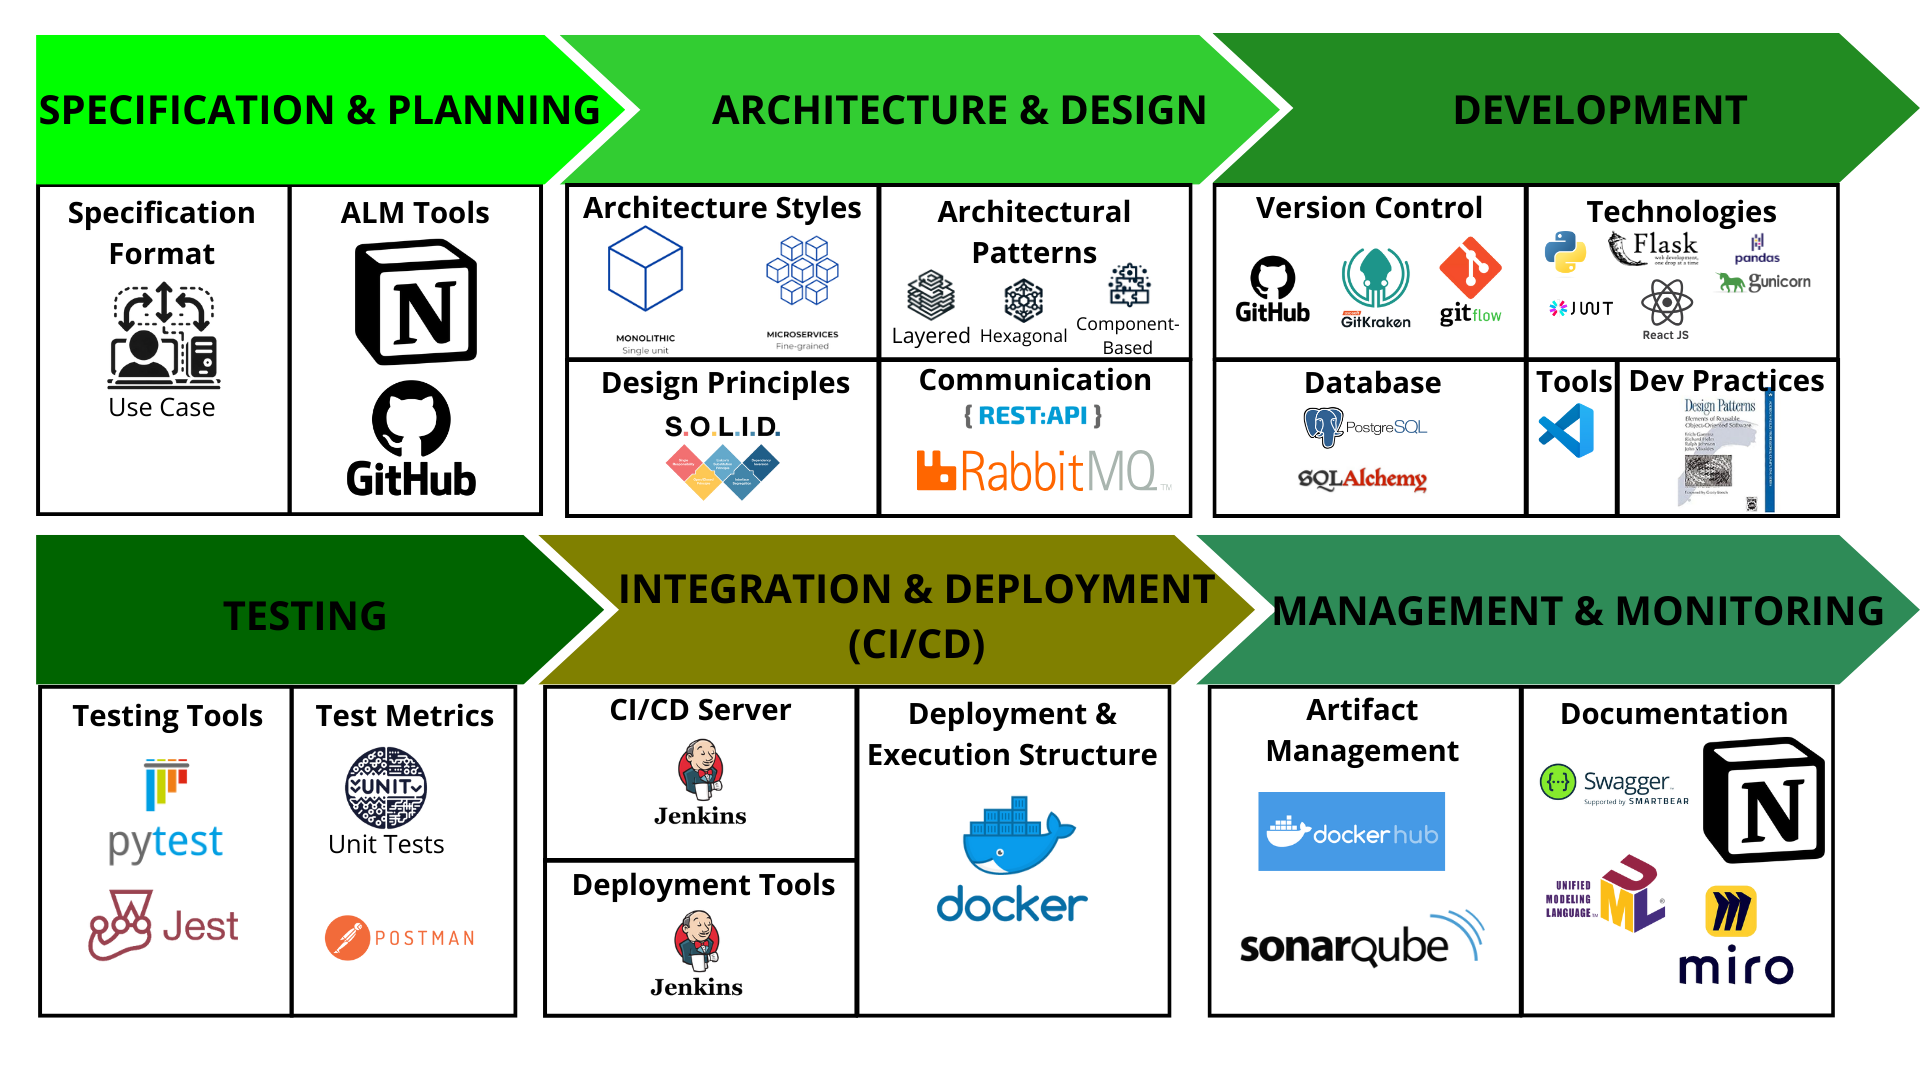
\includegraphics[width=1\linewidth]{Textuais/FinTrackr.png}
	\caption{tecnologias, técnicas, design, estilo arquiteturas}
	\label{fig:fintrackr_technologies}
\end{figure}

\section{Requisitos}

\subsection{Requisitos Funcionais}
\begin{enumerate}
	\item \textbf{RF01}: Implementação de um sistema de autenticação robusto e seguro, permitindo registro, login, recuperação de senha e gerenciamento de perfil.
	\item \textbf{RF02}: Facilitar o gerenciamento de informações do perfil do usuário, incluindo visualização, adição, atualização e exclusão de dados como nome, endereço e telefone.
	\item \textbf{RF03}: Permitir o registro de transações financeiras, categorizando-as como receitas ou despesas e associando detalhes pertinentes.
	\item \textbf{RF04}: Habilitar a criação, edição e exclusão de categorias de transações, associando detalhes como nome, cor e ícone.
	\item \textbf{RF05}: Proporcionar a definição e monitoramento de orçamentos mensais por categoria, mostrando gastos realizados e disponíveis.
	\item \textbf{RF06}: Prover um dashboard que apresente um resumo financeiro, incluindo saldo em contas, resumo de orçamentos, gastos por categoria e balanço geral.
	\item \textbf{RF07}: Integrar com um microserviço para permitir a importação de faturas bancárias em formato .csv, iniciando pelo Bradesco.
	\item \textbf{RF08}: Facilitar o gerenciamento de cartões de crédito, incluindo registro de faturas e lançamentos associados.
	\item \textbf{RF09}: Oferecer uma visualização detalhada do histórico de saldo, mostrando a evolução financeira do usuário.
	\item \textbf{RF10}: Permitir o registro e gerenciamento de bancos associados às contas do usuário.
\end{enumerate}

\subsection{Requisitos Não Funcionais}
\begin{enumerate}
	\item \textbf{RNF01}: A interface do sistema deve ser intuitiva e organizada.
	\item \textbf{RNF02}: Adaptabilidade para diferentes dispositivos, mantendo funcionalidade e design em smartphones, tablets e desktops.
	\item \textbf{RNF03}: Fornecer feedback claro e direto ao usuário em todas as interações.
	\item \textbf{RNF04}: Código-fonte bem estruturado, seguindo padrões reconhecidos de programação.
	\item \textbf{RNF05}: As operações do sistema devem ser otimizadas para resposta rápida, garantindo eficiência.
\end{enumerate}

\section{Regras de Negócio}
\begin{enumerate}
	\item \textbf{RN01}: Transações devem ser associadas a uma categoria.
	\item \textbf{RN02}: Cartões e contas com faturas ou transações associadas não podem ser excluídos.
	\item \textbf{RN03}: Categorias com transações associadas não podem ser excluídas.
	\item \textbf{RN04}: Ao dividir despesas em múltiplas categorias, o valor associado a cada categoria deve ser especificado.
	\item \textbf{RN05}: O total de valores associados em uma transação dividida entre categorias deve igualar o valor total da transação.
	\item \textbf{RN06}: Orçamentos não podem ter valores negativos.
	\item \textbf{RN07}: Despesas em cartões de crédito devem ser associadas à fatura corrente.
	\item \textbf{RN08}: Transações em contas impactam o saldo da mesma.
	\item \textbf{RN09}: Transações não podem ter datas futuras.
	\item \textbf{RN10}: Importações de faturas via .csv devem permitir edição pós-importação.
	\item \textbf{RN11}: Faturas de cartões possuem status baseados em datas de vencimento e pagamentos.
	\item \textbf{RN12}: Usuários devem ser notificados ao atingir ou exceder orçamentos.
	\item \textbf{RN13}: Categorias não podem ser duplicadas em uma transação dividida.
	\item \textbf{RN14}: Saldos negativos em contas devem ser prevenidos, a menos que permitidos.
	\item \textbf{RN15}: Informações de cartões ou contas duplicadas não são permitidas.
	\item \textbf{RN16}: Os usuários devem fornecer um email e senha válidos para se autenticar no sistema.
	\item \textbf{RN17}: Senhas devem ter um mínimo de 8 caracteres e conter pelo menos uma letra maiúscula, uma letra minúscula, um número e um caractere especial.
	\item \textbf{RN18}: Para recuperação de senha, o usuário deve confirmar sua identidade através de um link enviado ao seu email registrado.
	\item \textbf{RN19}: O email fornecido pelo usuário durante o registro ou atualização do perfil deve ser único no sistema.
	\item \textbf{RN20}: Para alterar a senha, o usuário deve fornecer a senha atual para confirmação.
\end{enumerate}

\section{Casos de Uso}

\subsection*{UC01: Autenticação no Sistema}
Apêndice \ref{apendiceUC01}

\subsection*{UC02: Gerenciar Perfil}
Apêndice \ref{apendiceUC02}

\subsection*{UC03: Registrar e Categorizar Transações}
Apêndice \ref{apendiceUC03}

\subsection*{UC04: Gerenciar Categorias}
Apêndice \ref{apendiceUC04}

\subsection*{UC05: Gerenciar Orçamentos}
Apêndice \ref{apendiceUC05}

\subsection*{UC06: Visualizar Dashboard Financeiro}
Apêndice \ref{apendiceUC06}

\subsection*{UC07: Importar Faturas}
Apêndice \ref{apendiceUC07}

\subsection*{UC08: Gerenciar Cartões e Faturas}
Apêndice \ref{apendiceUC08}

\subsection*{UC09: Acompanhar Evolução de Saldo}
Apêndice \ref{apendiceUC09}

\subsection*{UC10: Gerenciar Bancos}
Apêndice \ref{apendiceUC10}

\subsection*{UC11: Definir Mês de Referência para Transações}
Apêndice \ref{apendiceUC11}

\chapter{Especificação/Análise da Aplicação}

\section{Formato de especificação}

\begin{table}[ht]
	\centering
	\resizebox{\textwidth}{!}{%
		\begin{tabular}{|c|c|c|c|}
			\hline
			\multirow{2}{*}{\textbf{Critério}}     & \multicolumn{3}{c|}{\textbf{Formato de Especificação}}                                                                          \\ \cline{2-4}
			                                       & \textbf{Casos de Uso}                                  & \textbf{Casos de Uso 2.0}           & \textbf{Histórias de Usuário}    \\ \hline

			\multirow{2}{*}{\textbf{Quando Usar}}  & Projetos que necessitam                                & Quando você precisa de um           & Desenvolvimento Ágil,            \\
			                                       & de uma visão abrangente                                & formato estruturado e iterativo,    & projetos menores a médios,       \\
			                                       & e detalhada do sistema.                                & adaptável a mudanças.               & ou quando o foco está nas        \\
			                                       &                                                        &                                     & necessidades do usuário final.   \\ \hline

			\multirow{4}{*}{\textbf{Benefícios}}   & Oferece alto nível de                                  & Oferece uma estrutura               & Simples, focado,                 \\
			                                       & detalhamento e uma visão                               & detalhada, é iterativo,             & altamente adaptável a mudanças,  \\
			                                       & abrangente do sistema.                                 & flexível e adaptável.               & fácil de aprender e usar,        \\
			                                       &                                                        &                                     & e com baixo custo de manutenção. \\ \hline

			\multirow{4}{*}{\textbf{Desvantagens}} & Pode ser complexo e                                    & Requer planejamento cuidadoso       & Pode ser simplista               \\
			                                       & demorado para desenvolver                              & e tem custo de manutenção moderado. & para funcionalidades complexas.  \\
			                                       & e manter. Ideal para                                   &                                     &                                  \\
			                                       & sistemas maiores.                                      &                                     &                                  \\ \hline
		\end{tabular}%
	}
	\caption{Comparação revisada entre Casos de Uso, Casos de Uso 2.0 e Histórias de Usuário}
	\label{tab:revised_comparison}
\end{table}

O projeto \textit{Fintrackr}, embora seja de pequeno porte, tem uma complexidade inerente que demanda uma visão mais detalhada e estruturada do sistema. Neste cenário, os \textit{Casos de Uso} surgem como o formato de especificação ideal. A abordagem de Casos de Uso permite uma representação mais profunda das interações do sistema, alinhando-se perfeitamente com a Clean Architecture ao focar nas interações e nos fluxos de negócios.

Os Casos de Uso oferecem uma representação clara das funções e interações do sistema, facilitando a comunicação entre desenvolvedores, stakeholders e usuários. Esta abordagem detalhada garante que todas as nuances e requisitos do \textit{Fintrackr} sejam capturados e desenvolvidos de forma eficaz. Ao adotar Casos de Uso, garantimos uma compreensão profunda das necessidades do usuário e uma implementação sistemática dessas necessidades.

\section{Ferramentas de ALM}

\begin{table}[ht]
	\centering
	\resizebox{\textwidth}{!}{%
		\begin{tabular}{|c|c|c|c|c|}
			\hline
			\multirow{2}{*}{\textbf{Critério}}     & \multicolumn{4}{c|}{\textbf{Ferramenta}}                                                                              \\ \cline{2-5}
			                                       & \textbf{Jira}                            & \textbf{Trello}        & \textbf{Tuleap}       & \textbf{GitLab}           \\ \hline

			\multirow{2}{*}{\textbf{Quando Usar}}  & Projetos ágeis,                          & Projetos simples,      & Desenvolvimento ágil, & Desenvolvimento e         \\
			                                       & de médio a grande porte.                 & visualização Kanban.   & integração contínua.  & integração contínua.      \\
			                                       &                                          &                        & projetos open source. &                           \\ \hline

			\multirow{4}{*}{\textbf{Benefícios}}   & Flexível, integrações                    & Simples, intuitivo,    & Open source,          & Integração contínua,      \\
			                                       & amplas, poderoso.                        & flexível.              & personalizável.       & gestão de código.         \\
			                                       &                                          &                        &                       & gerenciamento de projeto. \\
			                                       &                                          &                        &                       &                           \\ \hline

			\multirow{4}{*}{\textbf{Desvantagens}} & Curva de aprendizado                     & Pode ser simplista     & Pode ser complexo     & Pode ser sobrecarregado   \\
			                                       & íngreme, pode ser caro.                  & para grandes projetos. & para novatos.         & para projetos menores.    \\
			                                       &                                          &                        &                       &                           \\
			                                       &                                          &                        &                       &                           \\ \hline
		\end{tabular}%
	}
	\caption{Comparação entre Jira, Trello, Tuleap e GitLab}
	\label{tab:tool_comparison}
\end{table}

Dada a natureza do projeto \textit{Fintrackr}, a seleção de ferramentas para gerenciamento e desenvolvimento é crucial. O Trello, com sua versão gratuita e simplicidade, surge como uma escolha primordial. Nossa equipe já possui familiaridade com o Trello, facilitando sua integração ao fluxo de trabalho. Além disso, adotamos um \href{https://github.com/ThiagoSchumann/fintrackr-docs}{repositório no GitHub} para centralizar documentação e artefatos, oferecendo uma visão unificada do projeto. Essa combinação de Trello e GitHub é ideal para as necessidades do \textit{Fintrackr}.


\section{Planejamento do desenvolvimento}

\section{Backlog}
%Thiago

\chapter{Definição da Arquitetura}

\noindent
\textbf{Architecture Decision Record (ADR)}

As ADRs (Documentos de Decisão de Arquitetura) implementadas neste projeto foram desenvolvidas seguindo o modelo proposto por Michael Nygard, disponível no \href{https://github.com/joelparkerhenderson/architecture-decision-record/blob/main/locales/en/templates/decision-record-template-by-michael-nygard/index.md}{GitHub}. Este modelo fornece uma estrutura clara e concisa para documentar decisões arquiteturais cruciais, garantindo consistência e compreensibilidade em todo o projeto.


\subsection{Estilo de Arquitetura}

\subsubsection*{ADR-001 - Tentativa de Implementar Todo o Projeto do \textit{Fintrackr} Usando Microserviços}
Apêndice \ref{apendiceADR001}

\subsubsection*{ADR-002 - Adoção de Arquitetura Monolítica para a Lógica de Negócios Principal do \textit{Fintrackr}}
Apêndice \ref{apendiceADR002}

\subsubsection*{ADR-003 - Criação de Microserviço Especializado para Processamento de Planilhas no \textit{Fintrackr}}
Apêndice \ref{apendiceADR003}

\subsubsection*{ADR-004 - Adoção de Arquitetura Monolítica no Front-end do \textit{Fintrackr}}
Apêndice \ref{apendiceADR004}


\subsection{Padrões Arquiteturais}

\subsubsection*{ADR-005 - Front-end React - Component-Based Architecture}
Apêndice \ref{apendiceADR005}

\subsubsection*{ADR-006 - Back-end Flask - Camadas com Clean/Onion}
Apêndice \ref{apendiceADR006}

\subsubsection*{ADR-007 - Microserviço com Pandas - Hexagonal}
Apêndice \ref{apendiceADR007}

\subsection{SOLID}

\subsubsection*{S - Single Responsibility Principle (Princípio da Responsabilidade Única)}
Sugere que uma classe ou módulo deve ter apenas uma razão para mudar, ou seja, deve ter apenas uma responsabilidade. Isso facilita a manutenção, testabilidade e compreensão do código. Dentro da arquitetura em camadas e do modelo Clean/Onion, é vital que cada camada ou serviço do FinTrackr tenha uma responsabilidade clara. Por exemplo, no contexto de um monólito, a camada de acesso a dados deve focar estritamente na persistência e recuperação de dados, enquanto a lógica de negócios reside em uma camada separada, desacoplada de detalhes específicos de banco de dados ou da apresentação.

\subsubsection*{O - Open/Closed Principle (Princípio do Aberto/Fechado)}
Propõe que entidades de software (como classes ou módulos) devem estar abertas para extensão, mas fechadas para modificação. Isso permite que novas funcionalidades sejam adicionadas sem alterar o código existente. Na arquitetura Clean/Onion, a lógica central do FinTrackr deve ser projetada de forma que novas funcionalidades ou regras de negócios possam ser adicionadas sem alterar o núcleo existente. Isso é especialmente útil em um ambiente de microserviços, onde novos serviços podem ser introduzidos sem perturbar os já existentes.

\subsubsection*{L - Liskov Substitution Principle (Princípio da Substituição de Liskov)}
Estabelece que subtipos devem ser substituíveis por seus tipos-base sem alterar a correção do programa. Independentemente da arquitetura adotada, seja monolítica ou baseada em microserviços, é crucial garantir que qualquer extensão ou modificação de entidades respeite este princípio. Por exemplo, se o FinTrackr introduzir uma nova variação de uma conta, qualquer instância dessa variação deve ser tratável como uma "conta" no sistema.

\subsubsection*{I - Interface Segregation Principle (Princípio da Segregação de Interfaces)}
Sugere que nenhuma classe deve ser forçada a implementar interfaces das quais não precisa. Na arquitetura Clean/Onion, isso se traduz em criar contratos claros e específicos entre as camadas, garantindo que a lógica de negócios se comunique apenas com as operações de que realmente precisa. Em uma abordagem de microserviços, cada serviço deve expor apenas as operações relevantes para seu domínio.

\subsubsection*{D - Dependency Inversion Principle (Princípio da Inversão de Dependência)}
Propõe que módulos de alto nível não devem depender de módulos de baixo nível, mas ambos devem depender de abstrações. Na arquitetura Clean/Onion, a lógica de negócios no núcleo não deve depender diretamente de detalhes externos, como bancos de dados ou APIs. Isso se alinha bem com o uso de ORMs, que fornecem uma abstração sobre o banco de dados. Em uma abordagem de microserviços, os serviços devem comunicar-se por meio de contratos bem definidos.



\subsection{Design Patterns}

\subsection*{Padrão Observer para a camada Transação}

\subsubsection*{Funcionamento}
O padrão Observer é um padrão comportamental que define uma dependência entre objetos de modo que quando um objeto muda de estado, todos os seus dependentes são notificados e atualizados automaticamente. O padrão é composto por um \textit{Subject} que mantém uma lista de seus dependentes, chamados \textit{Observers}, e os notifica sobre quaisquer mudanças de estado.

\subsubsection*{Aplicação ao FinTrackr}
No contexto do FinTrackr, o módulo "Transação" atua como o \textit{Subject}. Sua responsabilidade é notificar os usuários sobre transações que vencem no dia atual. Os módulos "Notificações por E-mail", "Notificações Push" e "Alertas no Dashboard" atuam como \textit{Observers}. Diariamente, o sistema verifica todas as transações com vencimento no dia atual e, para cada transação identificada, o módulo "Transação" notifica todos os observadores registrados.

\subsection*{Padrão Strategy para Importação de Faturas}

\subsubsection*{Funcionamento}
O padrão Strategy define uma família de algoritmos, encapsula cada um deles e os torna intercambiáveis. Esse padrão permite que o algoritmo varie independentemente dos clientes que o utilizam, promovendo uma separação entre a definição de estratégias e sua execução no contexto.

\subsubsection*{Aplicação ao FinTrackr}
No microserviço de "Importação de Faturas" do FinTrackr, o padrão Strategy é implementado por meio de uma interface chamada \textit{ImportStrategy}. Essa interface define um contrato comum para todos os algoritmos de importação. Implementações concretas, como \textit{BradescoImportStrategy}, definem algoritmos específicos para diferentes bancos. Quando uma requisição de importação é recebida, o microserviço determina qual estratégia usar e processa a importação conforme definido por essa estratégia.

\subsection{Padrões de comunicação}

\subsubsection*{ADR-008 - Adoção da Arquitetura REST para Comunicação entre Front-end e Back-end Flask}

Apêndice \ref{apendiceADR008}

\subsubsection*{ADR-009 - Adoção da Arquitetura REST para Comunicação entre Microserviços}

Apêndice \ref{apendiceADR009}

\subsubsection*{ADR-010 - Adoção do SQLAlchemy para Comunicação com o Banco de Dados no Flask}  

Apêndice \ref{apendiceADR010}
\chapter{Pipeline de CI/CD}

\section{Ferramenta de versionamento}

\begin{table}[ht]
	\centering
	\resizebox{\textwidth}{!}{%
		\begin{tabular}{|c|c|c|c|}
			\hline
			\multirow{2}{*}{\textbf{Plataforma}} & \multicolumn{3}{c|}{\textbf{Comparação}}                                                                          \\ \cline{2-4}
			                                     & \textbf{GitHub}                          & \textbf{GitLab}             & \textbf{Bitbucket}                       \\ \hline

			\multirow{2}{*}{\textbf{Benefícios}}
			                                     & Comunidade ampla,                        & CI/CD integrado,            & Integração Atlassian,                    \\
			                                     & Marketplace extenso.                     & Privacidade gratuita.       & Repositórios privados gratuitos.         \\ \hline

			\multirow{2}{*}{\textbf{Desvantagens}}
			                                     & Preço por repositório privado,           & Interface menos intuitiva,  & Limitações em repositórios gratuitos,    \\
			                                     & Limitações de armazenamento.             & Recursos de hardware.       & Menos recursos de CI/CD.                 \\ \hline

			\multirow{2}{*}{\textbf{Uso Comum}}
			                                     & Projetos open-source,                    & Solução completa de DevOps, & Equipes usando Atlassian.                \\
			                                     & Colaboração em larga escala.             & Controle total sobre CI/CD. & Integração de gerenciamento de projetos. \\ \hline
		\end{tabular}%
	}
	\caption{Comparação entre GitHub, GitLab e Bitbucket}
	\label{tab:platform_comparison}
\end{table}

\par Será utilizado o GitHub para controle de versões e colaboração eficiente no desenvolvimento de software. Ele fornece um ambiente centralizado para armazenar, acompanhar e gerenciar código-fonte, facilita a colaboração de equipes distribuídas e ajuda a controlar mudanças e atualizações no código, tornando o processo de desenvolvimento mais organizado, transparente e eficaz.

\section{Servidor de CI/CD}
\begin{table}[ht]
	\centering
	\resizebox{\textwidth}{!}{%
		\begin{tabular}{|c|c|c|c|c|}
			\hline
			\multirow{2}{*}{\textbf{Critério}} & \multicolumn{4}{c|}{\textbf{Servidor de CI/CD}}                                                                                     \\ \cline{2-5}
			                                   & \textbf{Jenkins}                                & \textbf{TravisCI}         & \textbf{CircleCI}      & \textbf{AWS CodePipeline}    \\ \hline

			\textbf{Quando Usar}               & Projetos grandes com                            & Projetos open-source      & Projetos pequenos      & Projetos na AWS              \\
			                                   & necessidade de customização.                    & com diferentes ambientes. & com integração rápida. & com serviços AWS integrados. \\ \hline

			\textbf{Benefícios}                & Alta customização,                              & Integração rápida,        & Integração rápida,     & Integração com               \\
			                                   & pipelines codificáveis.                         & fácil configuração.       & fácil configuração.    & serviços AWS.                \\ \hline

			\textbf{Desvantagens}              & Complexo e demorado                             & Ideal para projetos       & Pode ser limitado para & Menos flexível com           \\
			                                   & para configurar.                                & menores.                  & projetos grandes.      & integrações de terceiros.    \\ \hline
		\end{tabular}%
	}
	\caption{Comparação entre Servidores de CI/CD}
	\label{tab:ci_cd_comparison}
\end{table}

A escolha do Jenkins como nossa ferramenta de CI/CD é estratégica devido à sua natureza de código aberto e à familiaridade preexistente da nossa equipe com ela. O caráter open source do Jenkins alinha-se com nosso valor de promover a transparência e flexibilidade, enquanto a familiaridade da equipe acelera a integração e minimiza a curva de aprendizado. Com uma comunidade ativa e um ecossistema robusto, o Jenkins oferece um ambiente confiável para automatizar nossos processos de desenvolvimento, tornando-se uma escolha sólida para nosso projeto.

\section{Tecnologia utilizada}
Com base na estrutura do projeto proposta, foi realizada uma divisão clara entre o front-end e o back-end, sendo este último subdividido em dois projetos distintos. O primeiro projeto back-end é um microserviço dedicado a manipular e calcular dados para a planilha do Bradesco, enquanto o segundo engloba o restante das funcionalidades do software. A tabela a seguir apresenta uma visão geral das tecnologias de programação que serão adotadas para cada segmento do sistema, destacando quando usar, os benefícios e as desvantagens associadas a cada escolha tecnológica.

\begin{table}[ht]
	\centering
	\resizebox{\textwidth}{!}{%
		\begin{tabular}{|c|c|c|c|}
			\hline
			\textbf{Segmento do Sistema} & \textbf{Tecnologia} & \textbf{Finalidade}                                            & \textbf{Benefícios}                            \\ \hline
			Back-end (Geral)             & Python com Flask    & Desenvolvimento do núcleo funcional do sistema.                & Desenvolvimento rápido, fácil de aprender.     \\ \hline
			Microserviço Planilha        & Python com Pandas   & Manipulação e cálculo de dados da planilha do Bradesco.        & Manipulação eficiente de dados, fácil de usar. \\ \hline
			Front-end                    & React               & Construção de interfaces de usuário interativas e responsivas. & Componentização, reutilização de código.       \\ \hline
		\end{tabular}%
	}
	\caption{Tecnologias Adotadas nos Segmentos do Sistema}
	\label{tab:technology_adoption}
\end{table}


Nesta tabela, especificamos as tecnologias que serão utilizadas em cada segmento do sistema, juntamente com o contexto de uso, os benefícios e as desvantagens de cada uma. O Python foi escolhido para o back-end devido à sua simplicidade e rapidez no desenvolvimento, com o Flask proporcionando um framework leve para construir o back-end geral, e o Pandas oferecendo poderosas capacidades de manipulação de dados para o microserviço da planilha. Por outro lado, o React foi selecionado para o front-end devido à sua eficácia em construir interfaces de usuário interativas e reutilizáveis.

\section{Ferramentas de Build}
A seleção de uma ferramenta adequada para gerenciamento de dependências e construção do projeto é crucial para a eficiência do processo de desenvolvimento. Maven, Gradle e Docker são três tecnologias populares, cada uma com suas peculiaridades. Maven é conhecido por sua simplicidade e reprodutibilidade, Gradle por sua flexibilidade e desempenho, enquanto Docker destaca-se na criação e distribuição de contêineres. A tabela abaixo apresenta uma comparação entre essas tecnologias, visando auxiliar na escolha consciente da ferramenta mais alinhada às necessidades do projeto.

\begin{table}[ht]
	\centering
	\resizebox{\textwidth}{!}{%
		\begin{tabular}{|c|c|c|c|}
			\hline
			\multirow{2}{*}{\textbf{Critério}} & \multicolumn{3}{c|}{\textbf{Tecnologia}}                                                                       \\ \cline{2-4}
			                                   & \textbf{Maven}                           & \textbf{Gradle}         & \textbf{Docker}                           \\ \hline

			\textbf{Quando Usar}               & Projetos com                             & Projetos que necessitam & Quando a criação e                        \\
			                                   & estruturação clara.                      & de flexibilidade.       & distribuição de contêineres é necessária. \\ \hline

			\textbf{Benefícios}                & Simplicidade,                            & Flexibilidade,          & Portabilidade,                            \\
			                                   & reprodutibilidade.                       & desempenho.             & isolamento.                               \\ \hline

			\textbf{Desvantagens}              & Menos flexível,                          & Curva de aprendizado    & Requer conhecimento                       \\
			                                   & pode ser lento.                          & inicial.                & em contêineres.                           \\ \hline
		\end{tabular}%
	}
	\caption{Comparação entre Maven, Gradle e Docker}
	\label{tab:technology_comparison}
\end{table}


\section{Definição de Ferramentas e Estrutura de Execução para Deploy}

A implantação eficaz do \textit{Fintrackr} é crucial para garantir uma experiência de usuário contínua e robusta. Para alcançar essa eficiência, adotamos um conjunto de ferramentas líderes de mercado e definimos uma estrutura de execução que prioriza a escalabilidade, consistência e facilidade de manutenção.

\section{Ferramentas para Deploy}

\begin{itemize}
	\item \textbf{Ansible}: Uma ferramenta de automação poderosa que usamos para o provisionamento e configuração. Com sua ampla gama de módulos, o Ansible não apenas configura nodes do Kubernetes e instala o Docker, mas também se integra perfeitamente com outros sistemas e ferramentas, garantindo uma implantação homogênea e sem problemas.

	\item \textbf{GitHub}: Escolhido para controle de versões, o GitHub nos permite colaborar eficientemente e manter um histórico detalhado de todas as mudanças no código, facilitando o rastreamento e a reversão, se necessário.

	\item \textbf{Jenkins}: Para a integração contínua e entrega contínua (CI/CD), adotamos o Jenkins devido à sua flexibilidade, ampla comunidade e capacidade de se integrar com uma variedade de outras ferramentas, incluindo o Ansible e o Kubernetes.
\end{itemize}

\section{Estrutura de Execução}

\begin{itemize}
	\item \textbf{Docker}: A contêinerização é fundamental na era moderna da computação em nuvem. O Docker nos permite encapsular nossa aplicação e todas as suas dependências em contêineres, garantindo uma execução consistente em todos os ambientes, desde o desenvolvimento até a produção.
\end{itemize}
\section{GitFlow}
O \textit{GitFlow} é uma estratégia de fluxo de trabalho do Git que define uma estrutura robusta para projetos, facilitando o desenvolvimento paralelo, a colaboração em equipe e o lançamento de versões estáveis. A estratégia é composta por várias \textit{branches} que têm propósitos específicos. A seguir, detalhamos essas \textit{branches} e suas interações:

\begin{itemize}
	\item \textbf{main}: Contém o código considerado como produção. Cada \textit{commit} nesta branch é uma nova versão de produção.

	\item \textbf{develop}: Atua como uma branch de integração para novos recursos e é o principal local de desenvolvimento contínuo.

	\item \textbf{feature branches}: Criadas a partir da branch \textit{develop}. São utilizadas para desenvolver novas funcionalidades sem afetar o código principal. Quando uma funcionalidade é concluída, um \textit{Pull Request} (PR) é criado para mesclar a \textit{feature branch} de volta à branch \textit{develop}.

	\item \textbf{hotfix branches}: Surgem a partir da branch \textit{main}. Destinadas para correções rápidas diretamente no código de produção. Quando uma correção é finalizada, PRs são abertos para integrar a \textit{hotfix branch} tanto na branch \textit{main} quanto na \textit{develop}.
\end{itemize}

Os \textit{Pull Requests} (PRs) desempenham um papel fundamental no GitFlow. Eles oferecem um ponto de revisão e teste, garantindo que o código seja de alta qualidade antes da integração. Esse processo de revisão é vital para a colaboração em equipe, permitindo que os membros da equipe revisem, comentem e testem as alterações propostas antes de serem incorporadas ao código base.

O GitFlow, com sua estrutura clara e regras definidas, ajuda as equipes a gerenciar e versionar seu código de forma eficaz, garantindo lançamentos estáveis e facilitando o desenvolvimento contínuo e a colaboração.

\begin{figure}[ht]
	\centering
	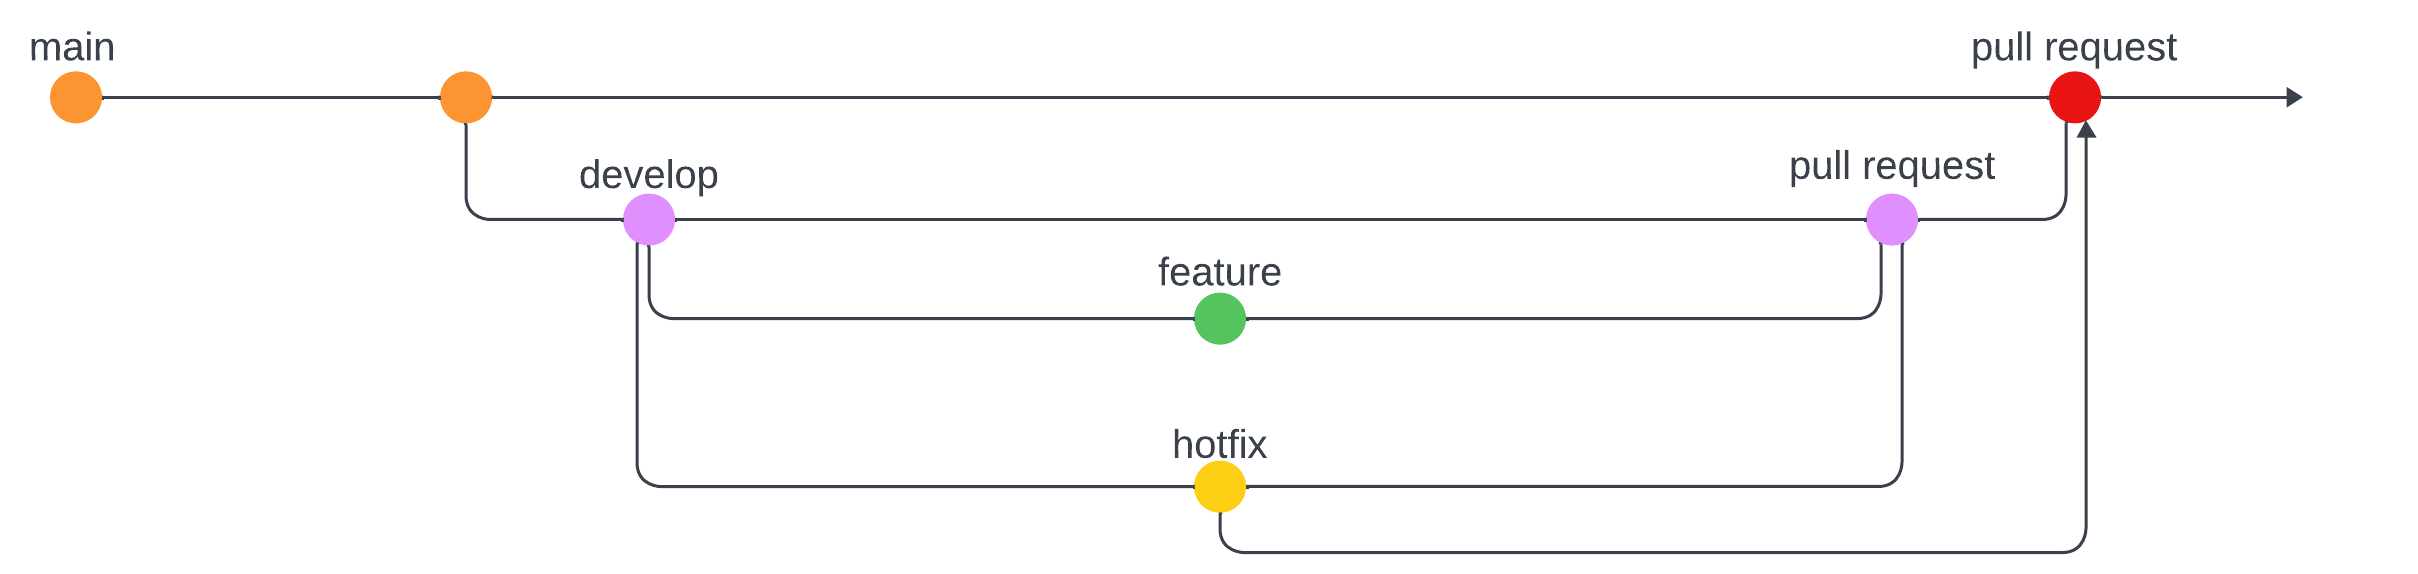
\includegraphics[width=1\linewidth]{Textuais/gitflow.png}
	\caption{\textit{GitFlow}}
	\label{fig:enter-label}
\end{figure}

\section{Testes}
\subsection{Ferramentas de Testes}

\par Para a linguagem Python será utilizado o Pytest, conhecido por sua sintaxe simples, identificação automática de testes, uso de fixtures, suporte a parametrização, extensibilidade por meio de plugins, e facilidade de integração com outras ferramentas de desenvolvimento. É amplamente adotado em projetos de código aberto e empresas, tornando o processo de teste eficiente e agradável para os desenvolvedores.

\par Para a linguagem React, será utilizado o Jest, ele é um framework de teste desenvolvido pelo Facebook que é amplamente usado na comunidade React. Ele é projetado para testar JavaScript, incluindo código React. O Jest é conhecido por sua simplicidade e integração perfeita com o React. Ele suporta testes de componentes, testes de unidades e testes de integração.

\subsection{Metrica de Cobertura de Testes}
\par A meta do nosso projeto é atingir uma cobertura de testes de 60\%. A cobertura de testes é fundamental para garantir a qualidade e a confiabilidade do nosso software. Com uma cobertura adequada, podemos identificar e corrigir erros de maneira eficaz, melhorar a manutenção do código e aumentar a confiança na estabilidade do sistema.
\par Para alcançar essa meta, planejamos implementar uma estratégia abrangente de testes que serão executados regularmente em um ambiente de integração contínua para garantir que nossa cobertura de testes seja mantida ao longo do tempo.
\par Atingir 60\% de cobertura de testes é um processo contínuo, e planejamos monitorar nosso progresso ao longo do ciclo de vida do projeto. Estabelecemos marcos específicos para avaliar nosso avanço e faremos ajustes conforme necessário para atender a essa meta.
\par Acreditamos que essa abordagem nos permitirá entregar um software de alta qualidade, com menos bugs e maior confiabilidade, beneficiando nossos usuários finais e nossa equipe de desenvolvimento

\section{Artefact Management}

\begin{table}[ht]
	\centering
	\resizebox{\textwidth}{!}{%
		\begin{tabular}{|c|c|c|c|c|}
			\hline
			\multirow{2}{*}{\textbf{Tecnologia}} & \multicolumn{4}{c|}{\textbf{Aspectos}}                                                                       \\ \cline{2-5}
			                                     & \textbf{Benefícios}                    & \textbf{Desvantagens} & \textbf{Uso Comum} & \textbf{Indicado Para} \\ \hline

			\textbf{Nexus}                       &
			- Gerenciamento de dependências.
			                                     &
			- Requer configuração.
			                                     &
			- Armazenamento de artefatos.
			                                     &
			- Projetos grandes.
			\\ \hline

			\textbf{DockerHub}                   &
			- Hospedagem de imagens Docker.
			                                     &
			- Limitações em repositórios públicos.
			                                     &
			- Distribuição de contêineres.
			                                     &
			- Projetos com Docker.
			\\ \hline

			\textbf{Sonar}                       &
			- Análise contínua da qualidade.
			                                     &
			- Configuração inicial.
			                                     &
			- Melhoria da qualidade do código.
			                                     &
			- Projetos com foco em qualidade.
			\\ \hline
		\end{tabular}%
	}
	\caption{Comparação entre Nexus, DockerHub, Sonar e Infraestrutura}
	\label{tab:technology_comparison}
\end{table}


\par Em nosso projeto, usaremos o SonarQube com o Docker, pois como vimos em sala é muito prático levantá-lo junto ao Docker, Ainda é muito  vantajoso porque permite analisar e melhorar a qualidade do código fonte, identificar vulnerabilidades de segurança, detectar bugs e defeitos, manter padrões de codificação consistentes, integrar análises de código ao pipeline de desenvolvimento, fornecer feedback imediato aos desenvolvedores, rastrear o histórico das análises, personalizar a configuração, gerar relatórios detalhados e, em última análise, aprimorar a qualidade do software. Isso contribui para a segurança, confiabilidade e desempenho de aplicativos em containers Docker.


\section{Documentação}
O Swagger é uma poderosa ferramenta para a construção de APIs RESTful, proporcionando uma suite completa para desenho, construção, documentação e uso de APIs. Ele fornece um conjunto de recursos que auxiliam os desenvolvedores a criar APIs consistentes, testáveis e padronizadas. Um dos componentes mais valiosos do Swagger é o Swagger UI, que fornece uma interface visual para interagir com a API, permitindo que os desenvolvedores e os usuários finais visualizem e testem as funcionalidades da API de forma intuitiva. No contexto do \textit{FinTrackr}, o Swagger será inestimável para documentar e testar as várias endpoints da API. Isso não só facilitará a integração entre o front-end e o back-end, mas também fornecerá uma referência clara para os desenvolvedores e partes interessadas sobre como a API funciona, quais dados ela aceita e quais respostas podem ser esperadas. Ao adotar o Swagger no \textit{FinTrackr}, garantimos uma abordagem padronizada e eficiente para a construção e documentação da API.


% -----------------------------------------------------------------
% ELEMENTOS PÓS-TEXTUAIS
% -----------------------------------------------------------------
\postextual

% Você pode comentar os elementos que não deseja em seu trabalho;

% Referências bibliográficas
\bibliography{Referencias}	% Elemento Obrigatório

% ----------------------------------------------------------
% Glossário
% ----------------------------------------------------------

%Consulte o manual da classe abntex2 para orientações sobre o glossário.

%\glossary




% ----------------------------------------------------------
% Glossário (Formatado Manualmente)
% ----------------------------------------------------------

%\chapter*{GLOSSÁRIO}
%\addcontentsline{toc}{chapter}{GLOSSÁRIO}

%{ \setlength{\parindent}{0pt} % ambiente sem indentação




%} % fim ambiente sem indentação


				% Elemento Opcional
% ----------------------------------------------------------
% Apêndices
% ----------------------------------------------------------

% ---
% Inicia os apêndices
% ---
\begin{apendicesenv}
	%\partapendices

	% ----------------------------------------------------------
\chapter{UC01 - Autenticação no Sistema}
% ----------------------------------------------------------
\label{apendiceUC01}
% Conteúdo do Apêndice UC01

\subsection*{Identificador}
\textit{UC01}

\subsection*{Título}
Autenticação no Sistema

\subsection*{Atores}
\begin{addmargin}[1.5cm]{0cm}
	\begin{itemize}
		\item Usuário
		\item Sistema de Autenticação
	\end{itemize}
\end{addmargin}

\subsection*{Pré-condições}
\begin{addmargin}[1.5cm]{0cm}
	\begin{itemize}
		\item O usuário possui acesso à interface de login.
	\end{itemize}
\end{addmargin}

\subsection*{Fluxo Principal}
\begin{addmargin}[1.5cm]{0cm}
	\begin{enumerate}
		\item O usuário acessa a página de login.
		\item O usuário insere seu email e senha.
		\item O sistema valida as credenciais.
		\item O usuário é autenticado e redirecionado para o dashboard.
	\end{enumerate}
\end{addmargin}

\subsection*{Fluxos Alternativos}
\begin{addmargin}[1.5cm]{0cm}
	\begin{itemize}
		\item \textbf{Registro de Novo Usuário}
		      \begin{enumerate}
		      	\item O usuário seleciona a opção para registrar-se.
		      	\item O sistema direciona o usuário para o formulário de registro.
		      	\item O usuário preenche os detalhes necessários e submete o formulário.
		      	\item O sistema valida as informações e cria uma nova conta.
		      	\item O usuário é redirecionado para a página de login.
		      \end{enumerate}
		          
		\item \textbf{Recuperação de Senha}
		      \begin{enumerate}
		      	\item O usuário seleciona a opção "Esqueceu a senha?".
		      	\item O sistema solicita o email do usuário.
		      	\item O usuário insere seu email e submete a solicitação.
		      	\item O sistema envia um link de recuperação de senha para o email do usuário.
		      \end{enumerate}
	\end{itemize}
\end{addmargin}

\subsection*{Fluxos de Exceção}
\begin{addmargin}[1.5cm]{0cm}
	\begin{itemize}
		\item \textbf{Credenciais Inválidas}
		      \begin{enumerate}
		      	\item O sistema detecta que o email ou senha inseridos estão incorretos.
		      	\item O sistema informa ao usuário sobre as credenciais inválidas.
		      \end{enumerate}
	\end{itemize}
\end{addmargin}

\subsection*{Pós-condições}
\begin{addmargin}[1.5cm]{0cm}
	\begin{itemize}
		\item O usuário obtém acesso às funcionalidades autenticadas do sistema.
	\end{itemize}
\end{addmargin}

\subsection*{Regras de Negócio}
\begin{addmargin}[1.5cm]{0cm}
	\begin{itemize}
		\item RN16: Os usuários devem fornecer um email e senha válidos para se autenticar no sistema.
		\item RN17: Senhas devem ter um mínimo de 8 caracteres e conter pelo menos uma letra maiúscula, uma letra minúscula, um número e um caractere especial.
	\end{itemize}
\end{addmargin}

\subsection*{Notas e Comentários}
\begin{addmargin}[1.5cm]{0cm}
	\begin{itemize}
		\item A interface de autenticação deve ser simples e intuitiva, minimizando erros de usuário.
	\end{itemize}
\end{addmargin}

	% ----------------------------------------------------------
\chapter{UC02 - Gerenciar Perfil}
% ----------------------------------------------------------
\label{apendiceUC02}

\subsection*{Identificador}
\textit{UC02}
% Conteúdo do Apêndice UC02

\subsection*{Título}
Gerenciar Perfil

\subsection*{Atores}
\begin{addmargin}[1.5cm]{0cm}
    \begin{itemize}
        \item Usuário
        \item Sistema de Gerenciamento de Perfil
    \end{itemize}
\end{addmargin}

\subsection*{Pré-condições}
\begin{addmargin}[1.5cm]{0cm}
    \begin{itemize}
        \item O usuário está autenticado no sistema.
    \end{itemize}
\end{addmargin}

\subsection*{Fluxo Principal}
\begin{addmargin}[1.5cm]{0cm}
    \begin{enumerate}
        \item O usuário acessa a seção de perfil.
        \item O sistema apresenta as informações atuais do perfil do usuário.
        \item O usuário seleciona a opção para editar o perfil.
        \item O usuário atualiza as informações desejadas e confirma as mudanças.
        \item O sistema valida e salva as alterações.
        \item O usuário é informado sobre o sucesso da atualização.
    \end{enumerate}
\end{addmargin}

\subsection*{Fluxos Alternativos}
\begin{addmargin}[1.5cm]{0cm}
    \begin{itemize}
        \item \textbf{Alterar Senha}:
        \begin{enumerate}
            \item O usuário seleciona a opção para alterar a senha.
            \item O sistema solicita a senha atual e a nova senha.
            \item O usuário insere as informações e confirma.
            \item O sistema valida a senha atual, aplica as regras de complexidade à nova senha e, se válido, atualiza a senha do usuário.
        \end{enumerate}
    \end{itemize}
\end{addmargin}

\subsection*{Fluxos de Exceção}
\begin{addmargin}[1.5cm]{0cm}
    \begin{itemize}
        \item \textbf{Dados Inválidos}:
        \begin{enumerate}
            \item Durante a atualização do perfil, o sistema detecta dados inválidos ou incompletos.
            \item O sistema informa ao usuário sobre os campos inválidos ou o que precisa ser corrigido.
        \end{enumerate}
    \end{itemize}
\end{addmargin}

\subsection*{Pós-condições}
\begin{addmargin}[1.5cm]{0cm}
    \begin{itemize}
        \item As informações do perfil do usuário são atualizadas no sistema.
    \end{itemize}
\end{addmargin}

\subsection*{Regras de Negócio}
\begin{addmargin}[1.5cm]{0cm}
    \begin{itemize}
        \item RN17: Senhas devem ter um mínimo de 8 caracteres e conter pelo menos uma letra maiúscula, uma letra minúscula, um número e um caractere especial.
        \item RN20: Para alterar a senha, o usuário deve fornecer a senha atual para confirmação.
    \end{itemize}
\end{addmargin}

\subsection*{Notas e Comentários}
\begin{addmargin}[1.5cm]{0cm}
    \begin{itemize}
        \item As informações do perfil devem ser tratadas com privacidade, e quaisquer alterações devem ser realizadas de forma segura.
    \end{itemize}
\end{addmargin}

	% ----------------------------------------------------------
\chapter{UC03 - Registrar e Categorizar Transações}
% ----------------------------------------------------------
\label{apendiceUC03}

\subsection*{Identificador}
\textit{UC03}

\subsection*{Título}
Registrar e Categorizar Transações

\subsection*{Atores}
\begin{addmargin}[1.5cm]{0cm}
	\begin{itemize}
		\item Usuário
		\item Sistema de Gestão Financeira
	\end{itemize}
\end{addmargin}

\subsection*{Pré-condições}
\begin{addmargin}[1.5cm]{0cm}
	\begin{itemize}
		\item O usuário está autenticado no sistema.
	\end{itemize}
\end{addmargin}

\subsection*{Fluxo Principal}
\begin{addmargin}[1.5cm]{0cm}
	\begin{enumerate}
		\item O usuário acessa a seção de transações.
		\item O usuário seleciona a opção para adicionar uma nova transação.
		\item O sistema apresenta o formulário de registro de transações.
		\item O usuário escolhe o tipo de transação: RegularTransaction ou CreditCardTransaction.
		\item O usuário insere os detalhes da transação, incluindo valor, tipo (receita ou despesa), data, descrição e, se for o caso, a fatura associada (para CreditCardTransaction).
		\item O usuário seleciona ou cria categorias para a transação.
		\item Se necessário, o usuário define o mês de referência para a transação.
		\item O sistema valida e registra a transação.
		\item O usuário é informado do sucesso do registro e a transação é exibida na lista de transações.
	\end{enumerate}
\end{addmargin}

\subsection*{Fluxos Alternativos}
\begin{addmargin}[1.5cm]{0cm}
	\begin{itemize}
		\item \textbf{Dividir Transação em Múltiplas Categorias}:
		      \begin{enumerate}
		      	\item Durante o registro da transação, o usuário opta por dividir a despesa em múltiplas categorias.
		      	\item O usuário especifica o valor associado a cada categoria.
		      	\item O sistema verifica se o total dos valores distribuídos corresponde ao valor total da transação.
		      	\item A transação é registrada com múltiplas categorias associadas.
		      \end{enumerate}
	\end{itemize}
\end{addmargin}

\subsection*{Fluxos de Exceção}
\begin{addmargin}[1.5cm]{0cm}
	\begin{itemize}
		\item \textbf{Valor da Transação Não Corresponde à Distribuição entre Categorias}:
		      \begin{enumerate}
		      	\item O sistema detecta que o valor total distribuído entre as categorias não corresponde ao valor total da transação.
		      	\item O usuário é informado do erro e solicitado a ajustar os valores.
		      \end{enumerate}
	\end{itemize}
\end{addmargin}

\subsection*{Pós-condições}
\begin{addmargin}[1.5cm]{0cm}
	\begin{itemize}
		\item A transação é registrada e categorizada, e reflete no saldo e relatórios do usuário.
	\end{itemize}
\end{addmargin}

\subsection*{Regras de Negócio}
\begin{addmargin}[1.5cm]{0cm}
	\begin{itemize}
		\item RN01: Transações devem ser associadas a uma categoria.
		\item RN05: O total de valores associados em uma transação dividida entre categorias deve igualar o valor total da transação.
		\item RN09: Transações não podem ter datas futuras.
		\item RN13: Categorias não podem ser duplicadas em uma transação dividida.
		\item RN23: Todas as transações devem ter um mês de referência para controle orçamentário.
	\end{itemize}
\end{addmargin}

\subsection*{Notas e Comentários}
\begin{addmargin}[1.5cm]{0cm}
	\begin{itemize}
		\item A interface de registro de transações deve ser simples e permitir a rápida inserção de múltiplas entradas.
	\end{itemize}
\end{addmargin}

	% ----------------------------------------------------------
\chapter{UC04 - Gerenciar Categorias}
% ----------------------------------------------------------
\label{apendiceUC04}

\subsection*{Identificador}
\textit{UC04}
% Conteúdo do Apêndice UC04

\subsection*{Título}
Gerenciar Categorias

\subsection*{Atores}
\begin{addmargin}[1.5cm]{0cm}
    \begin{itemize}
        \item Usuário
        \item Sistema de Gerenciamento de Categorias
    \end{itemize}
\end{addmargin}

\subsection*{Pré-condições}
\begin{addmargin}[1.5cm]{0cm}
    \begin{itemize}
        \item O usuário está autenticado no sistema.
    \end{itemize}
\end{addmargin}

\subsection*{Fluxo Principal}
\begin{addmargin}[1.5cm]{0cm}
    \begin{enumerate}
        \item O usuário acessa a seção de gerenciamento de categorias.
        \item O sistema apresenta a lista de categorias existentes.
        \item O usuário seleciona uma ação: criar nova categoria, editar categoria existente ou excluir categoria.
        \item O sistema executa a ação desejada e fornece feedback ao usuário.
    \end{enumerate}
\end{addmargin}

\subsection*{Fluxos Alternativos}
\begin{addmargin}[1.5cm]{0cm}
    \begin{itemize}
        \item \textbf{Criação de Nova Categoria}:
        \begin{enumerate}
            \item O usuário seleciona a opção para criar uma nova categoria.
            \item O sistema apresenta um formulário para inserção dos detalhes da categoria (nome, cor, ícone).
            \item O usuário preenche os detalhes e submete o formulário.
            \item O sistema valida as informações e cria a nova categoria.
        \end{enumerate}
        
        \item \textbf{Edição de Categoria Existente}:
        \begin{enumerate}
            \item O usuário seleciona uma categoria da lista.
            \item O sistema apresenta o formulário preenchido com os detalhes da categoria selecionada.
            \item O usuário altera as informações desejadas e submete o formulário.
            \item O sistema valida as alterações e atualiza a categoria.
        \end{enumerate}
    \end{itemize}
\end{addmargin}

\subsection*{Fluxos de Exceção}
\begin{addmargin}[1.5cm]{0cm}
    \begin{itemize}
        \item \textbf{Exclusão de Categoria Associada a Transações}:
        \begin{enumerate}
            \item O usuário tenta excluir uma categoria que possui transações associadas.
            \item O sistema detecta a associação e informa ao usuário que a categoria não pode ser excluída.
        \end{enumerate}
    \end{itemize}
\end{addmargin}

\subsection*{Pós-condições}
\begin{addmargin}[1.5cm]{0cm}
    \begin{itemize}
        \item As categorias são atualizadas conforme as ações realizadas pelo usuário.
    \end{itemize}
\end{addmargin}

\subsection*{Requisitos}
\begin{addmargin}[1.5cm]{0cm}
	\begin{itemize}
		\item \textbf{RF04}: Habilitar a criação, edição e exclusão de categorias de transações, associando detalhes como nome, cor e ícone.
	\end{itemize}
\end{addmargin}

\subsection*{Regras de Negócio}
\begin{addmargin}[1.5cm]{0cm}
    \begin{itemize}
        \item \textbf{RN01}: Transações devem ser associadas a uma categoria.
        \item \textbf{RN03}: Categorias com transações associadas não podem ser excluídas.
        \item \textbf{RN04}: Ao dividir despesas em múltiplas categorias, o valor associado a cada categoria deve ser especificado.
        \item \textbf{RN13}: Categorias não podem ser duplicadas em uma transação dividida.
    \end{itemize}
\end{addmargin}

\subsection*{Notas e Comentários}
\begin{addmargin}[1.5cm]{0cm}
    \begin{itemize}
        \item A interface de gerenciamento de categorias deve ser clara e intuitiva, permitindo a criação, edição e exclusão com facilidade.
    \end{itemize}
\end{addmargin}

	% ----------------------------------------------------------
\chapter{UC05 - Gerenciar Orçamentos}
% ----------------------------------------------------------
\label{apendiceUC05}

\subsection*{Identificador}
\textit{UC05}
% Conteúdo do Apêndice UC05

\subsection*{Título}
Gerenciar Orçamentos

\subsection*{Atores}
\begin{addmargin}[1.5cm]{0cm}
    \begin{itemize}
        \item Usuário
        \item Sistema de Gestão Financeira
    \end{itemize}
\end{addmargin}

\subsection*{Pré-condições}
\begin{addmargin}[1.5cm]{0cm}
    \begin{itemize}
        \item O usuário está autenticado e possui acesso à seção de orçamentos.
    \end{itemize}
\end{addmargin}

\subsection*{Fluxo Principal}
\begin{addmargin}[1.5cm]{0cm}
    \begin{enumerate}
        \item O usuário acessa a seção de orçamentos.
        \item O sistema exibe os orçamentos existentes categorizados por mês e categoria.
        \item O usuário seleciona um mês específico para visualizar ou editar.
        \item O sistema exibe detalhes do orçamento para o mês selecionado.
        \item O usuário pode adicionar, editar ou remover valores de orçamento para categorias específicas.
        \item O sistema valida e salva as alterações feitas pelo usuário.
    \end{enumerate}
\end{addmargin}

\subsection*{Fluxos Alternativos}
\begin{addmargin}[1.5cm]{0cm}
    \begin{itemize}
        \item \textbf{Criar Novo Orçamento}:
        \begin{enumerate}
            \item O usuário seleciona a opção para criar um novo orçamento.
            \item O sistema apresenta um formulário para inserir valores de orçamento por categoria.
            \item O usuário preenche os valores e submete.
            \item O sistema valida os dados e cria o novo orçamento.
        \end{enumerate}
    \end{itemize}
\end{addmargin}

\subsection*{Fluxos de Exceção}
\begin{addmargin}[1.5cm]{0cm}
    \begin{itemize}
        \item \textbf{Valores Negativos ou Inválidos}:
        \begin{enumerate}
            \item O sistema detecta valores negativos ou inválidos durante a edição ou criação de um orçamento.
            \item O sistema informa ao usuário sobre o erro e solicita correção.
        \end{enumerate}
    \end{itemize}
\end{addmargin}

\subsection*{Pós-condições}
\begin{addmargin}[1.5cm]{0cm}
    \begin{itemize}
        \item As alterações feitas pelo usuário nos orçamentos são salvas e refletidas no sistema.
    \end{itemize}
\end{addmargin}

\subsection*{Requisitos}
\begin{addmargin}[1.5cm]{0cm}
	\begin{itemize}
		\item \textbf{RF05}: Proporcionar a definição e monitoramento de orçamentos mensais por categoria, mostrando gastos realizados e disponíveis.
	\end{itemize}
\end{addmargin}

\subsection*{Regras de Negócio}
\begin{addmargin}[1.5cm]{0cm}
    \begin{itemize}
        \item \textbf{RN05}: Orçamentos não podem ter valores negativos.
        \item \textbf{RN12}: Usuários devem ser notificados ao atingir ou exceder orçamentos.
    \end{itemize}
\end{addmargin}

\subsection*{Notas e Comentários}
\begin{addmargin}[1.5cm]{0cm}
    \begin{itemize}
        \item A seção de orçamentos deve ser de fácil acesso e visualização, permitindo uma gestão rápida e eficiente dos valores.
    \end{itemize}
\end{addmargin}

	% ----------------------------------------------------------
\chapter{UC06 - Visualizar Dashboard Financeiro}
% ----------------------------------------------------------
\label{apendiceUC06}

\subsection*{Identificador}
\textit{UC06}

\subsection*{Título}
Visualizar Dashboard Financeiro

\subsection*{Atores}
\begin{addmargin}[1.5cm]{0cm}
    \begin{itemize}
        \item Usuário
        \item Sistema de Finanças
    \end{itemize}
\end{addmargin}

\subsection*{Pré-condições}
\begin{addmargin}[1.5cm]{0cm}
    \begin{itemize}
        \item O usuário está autenticado no sistema.
    \end{itemize}
\end{addmargin}

\subsection*{Fluxo Principal}
\begin{addmargin}[1.5cm]{0cm}
    \begin{enumerate}
        \item O usuário acessa a seção de dashboard.
        \item O sistema exibe o saldo total em contas.
        \item O sistema lista todas as contas com seus respectivos saldos e transações recentes.
        \item O sistema apresenta um resumo dos orçamentos definidos para o mês.
        \item O sistema mostra o total gasto por categoria.
        \item O sistema exibe um balanço geral de receitas versus despesas para o período selecionado.
    \end{enumerate}
\end{addmargin}

\subsection*{Fluxos Alternativos}
\begin{addmargin}[1.5cm]{0cm}
    \begin{itemize}
        \item \textbf{Exclusão de Conta do Saldo Total}:
        \begin{enumerate}
            \item O usuário seleciona uma ou mais contas para serem excluídas do saldo total.
            \item O sistema atualiza o saldo total exibido, excluindo as contas selecionadas.
        \end{enumerate}
    \end{itemize}
\end{addmargin}

\subsection*{Fluxos de Exceção}
\begin{addmargin}[1.5cm]{0cm}
    \begin{itemize}
        \item \textbf{Dados Indisponíveis}:
        \begin{enumerate}
            \item O sistema detecta um erro ao recuperar os dados financeiros do usuário.
            \item O sistema informa ao usuário sobre o erro e sugere que ele tente novamente mais tarde.
        \end{enumerate}
    \end{itemize}
\end{addmargin}

\subsection*{Pós-condições}
\begin{addmargin}[1.5cm]{0cm}
    \begin{itemize}
        \item O usuário tem uma visão clara e atualizada de sua situação financeira.
    \end{itemize}
\end{addmargin}

\subsection*{Requisitos}
\begin{addmargin}[1.5cm]{0cm}
	\begin{itemize}
		\item \textbf{RF06}: Prover um dashboard que apresente um resumo financeiro, incluindo saldo em contas, resumo de orçamentos, gastos por categoria e balanço geral.            
	\end{itemize}
\end{addmargin}

\subsection*{Regras de Negócio}
\begin{addmargin}[1.5cm]{0cm}
    \begin{itemize}
        \item \textbf{RN05}: O total de valores associados em uma transação dividida entre categorias deve igualar o valor total da transação.
        \item \textbf{RN06}: Orçamentos não podem ter valores negativos.
        \item \textbf{RN07}: Despesas em cartões de crédito devem ser associadas à fatura corrente.
        \item \textbf{RN08}: Transações em contas impactam o saldo da mesma.
        \item \textbf{RN09}: Transações não podem ter datas futuras.
    \end{itemize}
\end{addmargin}

\subsection*{Notas e Comentários}
\begin{addmargin}[1.5cm]{0cm}
    \begin{itemize}
        \item A interface do dashboard deve ser projetada para facilitar a compreensão rápida dos principais indicadores financeiros do usuário.
    \end{itemize}
\end{addmargin}

	% ----------------------------------------------------------
\chapter{UC07 - Importar Faturas}
% ----------------------------------------------------------
\label{apendiceUC07}

\subsection*{Identificador}
\textit{UC07}

\subsection*{Título}
Importar Faturas

\subsection*{Atores}
\begin{addmargin}[1.5cm]{0cm}
	\begin{itemize}
		\item Usuário
		\item Microserviço de Importação
	\end{itemize}
\end{addmargin}

\subsection*{Pré-condições}
\begin{addmargin}[1.5cm]{0cm}
	\begin{itemize}
		\item O usuário possui uma fatura no formato .csv para importar.
		\item O usuário está autenticado e tem permissão para importar faturas.
	\end{itemize}
\end{addmargin}

\subsection*{Fluxo Principal}
\begin{addmargin}[1.5cm]{0cm}
	\begin{enumerate}
		\item O usuário navega até a seção de importação de faturas.
		\item O usuário seleciona e carrega o arquivo .csv da fatura desejada.
		\item O sistema valida o formato e conteúdo do arquivo.
		\item O microserviço de importação processa o arquivo e extrai as transações.
		\item As transações são registradas no sistema associadas à conta ou cartão do usuário.
		\item O usuário é informado de que a importação foi bem-sucedida.
	\end{enumerate}
\end{addmargin}

\subsection*{Fluxos Alternativos}
\begin{addmargin}[1.5cm]{0cm}
	\begin{itemize}
		\item \textbf{Edição Pós-Importação}:
		      \begin{enumerate}
			      \item Após a importação bem-sucedida, o usuário opta por revisar as transações importadas.
			      \item O sistema apresenta uma lista das transações importadas.
			      \item O usuário edita ou exclui transações conforme necessário.
			      \item O sistema salva as alterações feitas pelo usuário.
		      \end{enumerate}
	\end{itemize}
\end{addmargin}

\subsection*{Fluxos de Exceção}
\begin{addmargin}[1.5cm]{0cm}
	\begin{itemize}
		\item \textbf{Arquivo Inválido}:
		      \begin{enumerate}
			      \item O sistema detecta que o arquivo .csv carregado é inválido ou corrompido.
			      \item O sistema informa ao usuário sobre o problema com o arquivo e solicita um novo arquivo.
		      \end{enumerate}
	\end{itemize}
\end{addmargin}

\subsection*{Pós-condições}
\begin{addmargin}[1.5cm]{0cm}
	\begin{itemize}
		\item As transações da fatura são registradas no sistema e podem ser visualizadas e gerenciadas pelo usuário.
	\end{itemize}
\end{addmargin}

\subsection*{Regras de Negócio}
\begin{addmargin}[1.5cm]{0cm}
	\begin{itemize}
		\item RN07: Despesas em cartões de crédito devem ser associadas à fatura corrente.
		\item RN10: Importações de faturas via .csv devem permitir edição pós-importação.
	\end{itemize}
\end{addmargin}

\subsection*{Notas e Comentários}
\begin{addmargin}[1.5cm]{0cm}
	\begin{itemize}
		\item A funcionalidade de importação deve suportar faturas de diferentes bancos, iniciando pelo Bradesco.
	\end{itemize}
\end{addmargin}

	% ----------------------------------------------------------
\chapter{UC08 - Gerenciar Cartões e Faturas}
% ----------------------------------------------------------
\label{apendiceUC08}

\subsection*{Identificador}
\textit{UC08}

\subsection*{Título}
Gerenciar Cartões e Faturas

\subsection*{Atores}
\begin{addmargin}[1.5cm]{0cm}
    \begin{itemize}
        \item Usuário
        \item Sistema de Gerenciamento Financeiro
    \end{itemize}
\end{addmargin}

\subsection*{Pré-condições}
\begin{addmargin}[1.5cm]{0cm}
    \begin{itemize}
        \item O usuário está autenticado e possui acesso à seção de gerenciamento de cartões.
    \end{itemize}
\end{addmargin}

\subsection*{Fluxo Principal}
\begin{addmargin}[1.5cm]{0cm}
    \begin{enumerate}
        \item O usuário acessa a seção de gerenciamento de cartões.
        \item O usuário visualiza seus cartões cadastrados.
        \item O usuário seleciona um cartão específico para visualizar detalhes e faturas associadas.
        \item O usuário pode adicionar, editar ou excluir informações do cartão.
        \item O usuário pode visualizar, adicionar, editar ou excluir faturas associadas ao cartão.
    \end{enumerate}
\end{addmargin}

\subsection*{Fluxos Alternativos}
\begin{addmargin}[1.5cm]{0cm}
    \begin{itemize}
        \item \textbf{Adicionar Novo Cartão}:
        \begin{enumerate}
            \item O usuário seleciona a opção para adicionar um novo cartão.
            \item O sistema apresenta um formulário para inserção de detalhes do cartão.
            \item O usuário preenche os detalhes e submete o formulário.
            \item O sistema valida as informações e adiciona o novo cartão à lista do usuário.
        \end{enumerate}
        
        \item \textbf{Excluir Cartão}:
        \begin{enumerate}
            \item O usuário seleciona um cartão e escolhe a opção para excluir.
            \item O sistema solicita confirmação.
            \item O usuário confirma a exclusão.
            \item O sistema remove o cartão e todas as faturas associadas.
        \end{enumerate}
    \end{itemize}
\end{addmargin}

\subsection*{Fluxos de Exceção}
\begin{addmargin}[1.5cm]{0cm}
    \begin{itemize}
        \item \textbf{Erro ao Adicionar Cartão}:
        \begin{enumerate}
            \item O sistema detecta um erro durante a adição do cartão (por exemplo, informações inválidas).
            \item O sistema informa ao usuário sobre o erro.
        \end{enumerate}
        
        \item \textbf{Erro ao Excluir Cartão}:
        \begin{enumerate}
            \item O sistema detecta um erro durante a exclusão do cartão (por exemplo, faturas pendentes).
            \item O sistema informa ao usuário sobre o erro.
        \end{enumerate}
    \end{itemize}
\end{addmargin}

\subsection*{Pós-condições}
\begin{addmargin}[1.5cm]{0cm}
    \begin{itemize}
        \item As informações do cartão e faturas associadas são atualizadas conforme as ações do usuário.
    \end{itemize}
\end{addmargin}

\subsection*{Regras de Negócio}
\begin{addmargin}[1.5cm]{0cm}
    \begin{itemize}
        \item RN02: Cartões e contas com faturas ou transações associadas não podem ser excluídos.
        \item RN07: Despesas em cartões de crédito devem ser associadas à fatura corrente.
        \item RN15: Informações de cartões ou contas duplicadas não são permitidas.
    \end{itemize}
\end{addmargin}

\subsection*{Notas e Comentários}
\begin{addmargin}[1.5cm]{0cm}
    \begin{itemize}
        \item A interface de gerenciamento de cartões deve oferecer uma visão clara de todas as informações e operações disponíveis.
    \end{itemize}
\end{addmargin}

	% ----------------------------------------------------------
\chapter{UC09 - Acompanhar Evolução de Saldo}
% ----------------------------------------------------------
\label{apendiceUC09}

\subsection*{Identificador}
\textit{UC09}

\subsection*{Título}
Acompanhar Evolução de Saldo

\subsection*{Atores}
\begin{addmargin}[1.5cm]{0cm}
	\begin{itemize}
		\item Usuário
		\item Sistema Financeiro
	\end{itemize}
\end{addmargin}

\subsection*{Pré-condições}
\begin{addmargin}[1.5cm]{0cm}
	\begin{itemize}
		\item O usuário está autenticado e possui acesso ao dashboard.
	\end{itemize}
\end{addmargin}

\subsection*{Fluxo Principal}
\begin{addmargin}[1.5cm]{0cm}
	\begin{enumerate}
		\item O usuário seleciona a opção para visualizar o histórico de saldo.
		\item O sistema apresenta uma representação gráfica (por exemplo, um gráfico de linhas) da evolução do saldo ao longo do tempo.
		\item O usuário pode selecionar diferentes intervalos de tempo (por exemplo, mês atual, últimos 6 meses, ano atual, etc.).
		\item O sistema atualiza a visualização com base no intervalo de tempo selecionado.
		\item O usuário pode interagir com o gráfico para obter detalhes específicos de datas e valores.
	\end{enumerate}
\end{addmargin}

\subsection*{Fluxos Alternativos}
\begin{addmargin}[1.5cm]{0cm}
	\begin{itemize}
		\item \textbf{Exportar Dados}:
		      \begin{enumerate}
			      \item O usuário seleciona a opção para exportar os dados do histórico de saldo.
			      \item O sistema oferece formatos de exportação (por exemplo, CSV, PDF).
			      \item O usuário seleciona o formato desejado e confirma.
			      \item O sistema gera e disponibiliza o arquivo para download.
		      \end{enumerate}
	\end{itemize}
\end{addmargin}

\subsection*{Fluxos de Exceção}
\begin{addmargin}[1.5cm]{0cm}
	\begin{itemize}
		\item \textbf{Sem Dados Suficientes}:
		      \begin{enumerate}
			      \item O sistema detecta que não há dados suficientes para exibir uma evolução significativa do saldo.
			      \item O sistema informa ao usuário sobre a falta de dados e sugere o registro de mais transações.
		      \end{enumerate}
	\end{itemize}
\end{addmargin}

\subsection*{Pós-condições}
\begin{addmargin}[1.5cm]{0cm}
	\begin{itemize}
		\item O usuário tem uma visão clara da evolução do seu saldo financeiro ao longo do tempo.
	\end{itemize}
\end{addmargin}

\subsection*{Regras de Negócio}
\begin{addmargin}[1.5cm]{0cm}
	\begin{itemize}
		\item RN08: Transações em contas impactam o saldo da mesma.
		\item RN09: Transações não podem ter datas futuras.
	\end{itemize}
\end{addmargin}

\subsection*{Notas e Comentários}
\begin{addmargin}[1.5cm]{0cm}
	\begin{itemize}
		\item A interface de visualização do histórico de saldo deve ser clara e proporcionar fácil interpretação dos dados.
	\end{itemize}
\end{addmargin}

	% ----------------------------------------------------------
\chapter{UC10 - Gerenciar Bancos}
% ----------------------------------------------------------
\label{apendiceUC10}

\subsection*{Identificador}
\textit{UC10}

\subsection*{Título}
Gerenciar Bancos

\subsection*{Atores}
\begin{addmargin}[1.5cm]{0cm}
	\begin{itemize}
		\item Usuário
		\item Sistema de Gerenciamento de Bancos
	\end{itemize}
\end{addmargin}

\subsection*{Pré-condições}
\begin{addmargin}[1.5cm]{0cm}
	\begin{itemize}
		\item O usuário está autenticado no sistema.
		\item O usuário possui acesso à seção de gerenciamento de bancos.
	\end{itemize}
\end{addmargin}

\subsection*{Fluxo Principal}
\begin{addmargin}[1.5cm]{0cm}
	\begin{enumerate}
		\item O usuário acessa a seção de gerenciamento de bancos.
		\item O sistema exibe a lista de bancos cadastrados pelo usuário.
		\item O usuário pode escolher adicionar, editar ou excluir informações de um banco.
		\item O sistema realiza a ação solicitada e atualiza a lista de bancos.
	\end{enumerate}
\end{addmargin}

\subsection*{Fluxos Alternativos}
\begin{addmargin}[1.5cm]{0cm}
	\begin{itemize}
		\item \textbf{Adicionar Novo Banco}:
		      \begin{enumerate}
			      \item O usuário seleciona a opção para adicionar um novo banco.
			      \item O sistema apresenta um formulário para inserção de detalhes do banco.
			      \item O usuário preenche os detalhes e submete o formulário.
			      \item O sistema valida as informações e adiciona o novo banco à lista.
		      \end{enumerate}

		\item \textbf{Editar Informações de um Banco Existente}:
		      \begin{enumerate}
			      \item O usuário seleciona um banco da lista e escolhe a opção para editar.
			      \item O sistema apresenta um formulário preenchido com as informações atuais do banco.
			      \item O usuário realiza as alterações desejadas e submete o formulário.
			      \item O sistema valida e atualiza as informações do banco.
		      \end{enumerate}
	\end{itemize}
\end{addmargin}

\subsection*{Fluxos de Exceção}
\begin{addmargin}[1.5cm]{0cm}
	\begin{itemize}
		\item \textbf{Informações do Banco Duplicadas}:
		      \begin{enumerate}
			      \item O sistema detecta que as informações inseridas para um novo banco ou após a edição já existem para outro banco registrado.
			      \item O sistema informa ao usuário sobre a duplicidade e solicita correção.
		      \end{enumerate}
	\end{itemize}
\end{addmargin}

\subsection*{Pós-condições}
\begin{addmargin}[1.5cm]{0cm}
	\begin{itemize}
		\item A lista de bancos do usuário é atualizada com as informações corretas.
	\end{itemize}
\end{addmargin}

\subsection*{Regras de Negócio}
\begin{addmargin}[1.5cm]{0cm}
	\begin{itemize}
		\item RN10: O email fornecido pelo usuário durante o registro ou atualização do perfil deve ser único no sistema.
		\item RN15: Informações de cartões ou contas duplicadas não são permitidas.
	\end{itemize}
\end{addmargin}

\subsection*{Notas e Comentários}
\begin{addmargin}[1.5cm]{0cm}
	\begin{itemize}
		\item O gerenciamento eficaz de informações bancárias é crucial para a integridade dos dados e a experiência do usuário.
	\end{itemize}
\end{addmargin}

	% ----------------------------------------------------------
\chapter{UC11 -  Definir Mês de Referência para Transações}
% ----------------------------------------------------------
\label{apendiceUC11}

\subsection*{Identificador}
\textit{UC11}

\subsection*{Título}
Definir Mês de Referência para Transações

\subsection*{Atores}
\begin{addmargin}[1.5cm]{0cm}
	\begin{itemize}
		\item Usuário
		\item Sistema de Gestão Financeira
	\end{itemize}
\end{addmargin}

\subsection*{Pré-condições}
\begin{addmargin}[1.5cm]{0cm}
	\begin{itemize}
		\item O usuário está autenticado no sistema.
		\item O usuário está registrando ou editando uma transação.
	\end{itemize}
\end{addmargin}

\subsection*{Fluxo Principal}
\begin{addmargin}[1.5cm]{0cm}
	\begin{enumerate}
		\item Durante o registro ou edição de uma transação, o usuário identifica a necessidade de definir um mês de referência.
		\item O sistema apresenta a opção para selecionar o mês de referência.
		\item O usuário seleciona o mês e ano desejados.
		\item O sistema valida a escolha.
		\item O mês de referência é associado à transação.
	\end{enumerate}
\end{addmargin}

\subsection*{Fluxos Alternativos}
\textit{N/A}

\subsection*{Fluxos de Exceção}
\textit{N/A}

\subsection*{Pós-condições}
\begin{addmargin}[1.5cm]{0cm}
	\begin{itemize}
		\item O mês de referência é definido para a transação, permitindo um controle orçamentário mais preciso.
	\end{itemize}
\end{addmargin}

\subsection*{Regras de Negócio}
\begin{addmargin}[1.5cm]{0cm}
	\begin{itemize}
		\item RN23: Todas as transações devem ter um mês de referência para controle orçamentário.
	\end{itemize}
\end{addmargin}

\subsection*{Notas e Comentários}
\begin{addmargin}[1.5cm]{0cm}
	\begin{itemize}
		\item A definição do mês de referência é especialmente crucial para transações de cartão de crédito, onde o impacto orçamentário pode não coincidir com a data da transação.
	\end{itemize}
\end{addmargin}

	
% ----------------------------------------------------------
\chapter{ADR-001 - Tentativa de Implementar Todo o Projeto do \textit{Fintrackr} Usando Microserviços}
% ----------------------------------------------------------
\label{apendiceADR001}
% Conteúdo do Apêndice ADR-001

\subsubsection*{Title}
Tentativa de Implementar Todo o Projeto do \textit{Fintrackr} Usando Microserviços.

\subsubsection*{Status}
Rejected - Devido ao tempo e à complexidade aumentada, decidiu-se não seguir essa abordagem.

\subsubsection*{Context}
O projeto \textit{Fintrackr} visa oferecer uma ferramenta robusta para o gerenciamento de finanças. Com o aumento da complexidade e a variedade de funcionalidades, considerou-se a possibilidade de utilizar uma abordagem totalmente baseada em microserviços.

\subsubsection*{Decision}
Tentar implementar todo o projeto do \textit{Fintrackr} usando uma arquitetura baseada em microserviços.

\subsubsection*{Consequences}
\begin{itemize}
	\item \textbf{Especialização}: Cada microserviço pode ser otimizado para sua função específica.
	\item \textbf{Flexibilidade}: Microserviços podem ser desenvolvidos, escalados ou modificados independentemente.
	\item \textbf{Resiliência}: Falhas em um microserviço não afetariam outros microserviços.
	\item \textbf{Complexidade Aumentada}: A gestão de múltiplos microserviços pode complicar o desenvolvimento e a manutenção.
\end{itemize}

	
% ----------------------------------------------------------
\chapter{ADR-002 - Adoção de Arquitetura Monolítica para a Lógica de Negócios Principal do \textit{Fintrackr}}
% ----------------------------------------------------------
\label{apendiceADR002}
% Conteúdo do Apêndice ADR-002

\subsubsection*{Title}
Adoção de Arquitetura Monolítica para a Lógica de Negócios Principal do \textit{Fintrackr}.

\subsubsection*{Status}
Accepted

\subsubsection*{Context}
O projeto \textit{Fintrackr} visa fornecer uma solução robusta para o gerenciamento de finanças. Uma parte significativa do sistema é composta por operações de cadastro e lógica de negócios. Para acomodar essas necessidades de maneira coesa, é essencial considerar uma abordagem arquitetural que possa integrar eficientemente esses componentes.

\subsubsection*{Decision}
Adotar uma arquitetura monolítica para a lógica de negócios principal e cadastros do \textit{Fintrackr}.

\subsubsection*{Consequences}
\begin{itemize}
	\item \textbf{Consistência}: Um monólito oferece uma base de código unificada, o que pode simplificar o desenvolvimento e a manutenção.
	\item \textbf{Performance}: Com todos os componentes principais no mesmo processo, as latências de comunicação são minimizadas.
	\item \textbf{Simplicidade}: Menos preocupações com a comunicação entre serviços.
	\item \textbf{Escalabilidade Vertical}: O monólito pode ser escalado verticalmente, mas pode haver limitações na escalabilidade horizontal.
	\item \textbf{Potencial de Acoplamento}: Pode haver riscos de acoplamento apertado entre os módulos ao longo do tempo.
	\item \textbf{Curva de aprendizado}: Desenvolvedores familiarizados com microserviços podem precisar de tempo para se adaptar à abordagem monolítica.
	\item \textbf{Flexibilidade}: Modificações no sistema podem requerer reimplantações completas em vez de serviços individuais.
	\item \textbf{Manutenção}: À medida que o projeto cresce, a manutenção pode se tornar mais desafiadora devido ao tamanho do código base.
\end{itemize}

	
% ----------------------------------------------------------
\chapter{ADR-003 - Criação de Microserviço Especializado para Processamento de Planilhas no \textit{Fintrackr}}
% ----------------------------------------------------------
\label{apendiceADR003}
% Conteúdo do Apêndice ADR-003

\subsubsection*{Title}
Criação de Microserviço Especializado para Processamento de Planilhas no \textit{Fintrackr}.

\subsubsection*{Status}
Accepted

\subsubsection*{Context}
O \textit{Fintrackr} tem uma necessidade específica de processar informações de planilhas, transformando-as em um formato desejado para integração com o sistema. Esta operação é distinta das funções de lógica de negócios principais e, portanto, requer uma abordagem arquitetural especializada.

\subsubsection*{Decision}
Criar um microserviço dedicado responsável por receber, processar e retornar informações de planilhas em um formato desejado.

\subsubsection*{Consequences}
\begin{itemize}
	\item \textbf{Especialização}: O microserviço pode ser otimizado para processar planilhas de forma eficiente.
	\item \textbf{Flexibilidade}: O microserviço pode ser desenvolvido, escalado ou modificado independentemente do monólito.
	\item \textbf{Isolamento}: Falhas ou problemas no microserviço não afetarão o funcionamento do monólito.
	\item \textbf{Complexidade Adicional}: Introduz a necessidade de gerenciar a comunicação entre o monólito e o microserviço.
	\item \textbf{Overhead de Rede}: A comunicação entre o monólito e o microserviço pode introduzir latências.
	\item \textbf{Curva de aprendizado}: Os desenvolvedores podem precisar de formação ou familiarização com a gestão de microserviços.
	\item \textbf{Gerenciamento}: Monitoramento, logging e rastreamento adicionais serão necessários para gerenciar o microserviço.
	\item \textbf{Integração}: Garantir uma integração robusta e eficiente com o monólito será crucial.
\end{itemize}

	
% ----------------------------------------------------------
\chapter{ADR-004 - Adoção de Arquitetura Monolítica no Front-end do \textit{Fintrackr}}
% ----------------------------------------------------------
\label{apendiceADR004}
% Conteúdo do Apêndice ADR-004

\subsubsection*{Title}
Adoção de Arquitetura Monolítica no Front-end do \textit{Fintrackr}.

\subsubsection*{Status}
Accepted

\subsubsection*{Context}
O projeto \textit{Fintrackr} busca fornecer uma solução eficaz para o gerenciamento de finanças. Dada a pouca experiência da equipe com o desenvolvimento de front-end e a necessidade de garantir uma rápida aprendizagem e eficiência no desenvolvimento, é crucial escolher uma abordagem arquitetural que seja familiar e minimamente complexa.

\subsubsection*{Decision}
Adotar uma arquitetura monolítica para o front-end do \textit{Fintrackr}.

\subsubsection*{Consequences}
\begin{itemize}
    \item \textbf{Simplicidade}: Um front-end monolítico é mais simples de entender, desenvolver e manter, especialmente para equipes menos experientes.
    \item \textbf{Integração Estreita}: Todos os componentes do front-end estarão estreitamente integrados, permitindo uma melhor coesão.
    \item \textbf{Menor Curva de Aprendizado}: A equipe pode se concentrar em desenvolver funcionalidades em vez de gerenciar a complexidade de múltiplos serviços ou componentes independentes.
    \item \textbf{Desafios de Escalabilidade}: À medida que o projeto cresce, pode haver desafios associados à escalabilidade e manutenção do front-end monolítico.
\end{itemize}

\newpage

	
% ----------------------------------------------------------
\chapter{ADR-005 - Front-end React - Component-Based Architecture}
% ----------------------------------------------------------
\label{apendiceADR005}
% Conteúdo do Apêndice ADR-005

\subsubsection*{Title}
Front-end React - Component-Based Architecture.

\subsubsection*{Status}
Accepted

\subsubsection*{Context}
O \textit{Fintrackr} visa fornecer uma interface de usuário intuitiva e eficiente para gerenciamento de finanças. A escolha da arquitetura do front-end é crucial para garantir uma experiência de usuário consistente e de alta qualidade.

\subsubsection*{Decision}
Adotar a arquitetura baseada em componentes usando o framework React para o front-end do \textit{Fintrackr}.

\subsubsection*{Consequences}
\begin{itemize}
	\item \textbf{Modularidade}: A arquitetura baseada em componentes permite modularidade, facilitando o desenvolvimento, teste e manutenção de partes individuais da interface do usuário.
	\item \textbf{Reusabilidade}: Componentes podem ser reutilizados em diferentes partes da aplicação ou até mesmo em outros projetos.
	\item \textbf{Eficiência}: Com o Virtual DOM do React, as atualizações da interface do usuário são otimizadas para serem rápidas e eficientes.
	\item \textbf{Comunidade}: React tem uma grande comunidade e ecossistema, oferecendo muitas bibliotecas e ferramentas auxiliares.
	\item \textbf{Curva de Aprendizado}: Pode haver uma curva de aprendizado para desenvolvedores não familiarizados com React ou arquitetura baseada em componentes.
	\item \textbf{Dependências}: Dependência de bibliotecas e ferramentas específicas do ecossistema React.
\end{itemize}

	
% ----------------------------------------------------------
\chapter{ADR-006 - Back-end Flask - Camadas com Clean/Onion}
% ----------------------------------------------------------
\label{apendiceADR006}
% Conteúdo do Apêndice ADR-006

\subsubsection*{Title}
Back-end Flask - Camadas com Clean/Onion.

\subsubsection*{Status}
Accepted

\subsubsection*{Context}
O \textit{Fintrackr} tem a responsabilidade de gerenciar a lógica de negócios relacionada ao gerenciamento de finanças. A escolha da arquitetura do back-end é essencial para garantir que a aplicação seja flexível, testável e manutenível.

\subsubsection*{Decision}
Adotar uma combinação de arquitetura em camadas com Clean/Onion para o back-end do \textit{Fintrackr} construído com Flask.

\subsubsection*{Consequences}
\begin{itemize}
	\item \textbf{Separação de Responsabilidades}: Esta abordagem garante que as responsabilidades sejam claramente separadas em diferentes camadas.
	\item \textbf{Flexibilidade}: Facilita mudanças e evolução do código ao manter a lógica de negócios separada da infraestrutura.
	\item \textbf{Testabilidade}: Torna mais fácil escrever testes unitários para a lógica de negócios.
	\item \textbf{Manutenibilidade}: O código torna-se mais fácil de manter e entender.
	\item \textbf{Curva de Aprendizado}: Pode haver uma curva de aprendizado para desenvolvedores não familiarizados com a arquitetura Clean/Onion.
	\item \textbf{Complexidade}: A introdução de várias camadas e a separação rigorosa podem aumentar a complexidade inicial.
\end{itemize}

\newpage

	
% ----------------------------------------------------------
\chapter{ADR-007 - Microserviço com Pandas - Hexagonal}
% ----------------------------------------------------------
\label{apendiceADR007}
% Conteúdo do Apêndice ADR-007

\subsubsection*{Title}
Microserviço com Pandas - Hexagonal.

\subsubsection*{Status}
Accepted

\subsubsection*{Context}
O \textit{Fintrackr} tem uma necessidade específica de processar dados de planilhas para integração com o sistema. Esta funcionalidade é distinta das funções principais da aplicação e pode necessitar de escalabilidade e adaptabilidade independentes.

\subsubsection*{Decision}
Adotar a arquitetura hexagonal para o microserviço especializado em processamento de dados com Pandas.

\subsubsection*{Consequences}
\begin{itemize}
	\item \textbf{Flexibilidade}: A arquitetura hexagonal permite que o microserviço seja facilmente adaptado para diferentes interfaces ou integrações no futuro.
	\item \textbf{Testabilidade}: Facilita a escrita de testes, pois a lógica de negócios é desacoplada dos adaptadores.
	\item \textbf{Isolamento}: Falhas ou problemas no microserviço não afetarão outras partes da aplicação.
	\item \textbf{Especialização}: O microserviço pode ser otimizado para processar planilhas de forma eficiente.
	\item \textbf{Curva de Aprendizado}: Pode haver uma curva de aprendizado para desenvolvedores não familiarizados com a arquitetura hexagonal.
	\item \textbf{Gerenciamento Adicional}: Requer monitoramento, logging e rastreamento adicionais para gerenciar o microserviço.
\end{itemize}

    % ----------------------------------------------------------
\chapter{ADR-008 - Adoção da Arquitetura REST para Comunicação entre Front-end e Back-end Flask}
% ----------------------------------------------------------
\label{apendiceADR008}
% Conteúdo do Apêndice ADR-008

\subsubsection*{Title}
Adoção da Arquitetura REST para Comunicação entre Front-end e Back-end Flask.

\subsubsection*{Status}
Accepted

\subsubsection*{Context}
O \textit{Fintrackr} possui componentes de front-end e um back-end construído com Flask. Para garantir uma comunicação eficiente e padronizada entre esses dois componentes, é necessário escolher uma arquitetura de comunicação apropriada.

\subsubsection*{Decision}
Adotar a arquitetura REST (Representational State Transfer) como a principal forma de comunicação entre o front-end e o back-end Flask do Fintrackr.

\subsubsection*{Consequences}
\begin{itemize}
	\item \textbf{Padronização}: A arquitetura REST fornece um conjunto padronizado de convenções para a criação de APIs.
	\item \textbf{Escalabilidade}: REST é stateless, o que facilita a escalabilidade horizontal do sistema.
	\item \textbf{Flexibilidade}: Permite que o front-end e o back-end Flask se comuniquem de maneira eficiente.
	\item \textbf{Interoperabilidade}: Facilita a integração com sistemas externos ou de terceiros.
	\item \textbf{Simplicidade e Eficiência}: REST utiliza os métodos HTTP padrão e é baseado em recursos, tornando-o intuitivo e eficiente.
	\item \textbf{Desacoplamento}: Permite que o front-end e o back-end Flask evoluam separadamente, desde que a API permaneça consistente.
	\item \textbf{Conformidade com Padrões da Web}: REST é amplamente adotado na web, e muitas ferramentas e bibliotecas suportam essa arquitetura.
	\item \textbf{Considerações de Segurança}: Como qualquer API exposta, medidas de segurança adequadas, como autenticação e autorização, devem ser implementadas ao comunicar entre o front-end e o back-end Flask.
\end{itemize}

	% ----------------------------------------------------------
\chapter{ADR-009 - Adoção do RabbitMQ para Comunicação entre o Microserviço da Planilha de Fatura e o Back-end Flask}
% ----------------------------------------------------------
\label{apendiceADR009}
% Conteúdo do Apêndice ADR-009

\subsubsection*{Title}
Adoção do RabbitMQ para Comunicação entre o Microserviço da Planilha de Fatura e o Back-end Flask.

\subsubsection*{Status}
Accepted

\subsubsection*{Context}
Para integrar o microserviço especializado da planilha de fatura com o back-end Flask do \textit{Fintrackr}, é crucial ter uma solução de mensageiria confiável que facilite a comunicação assíncrona, garanta a entrega de mensagens e suporte a escalabilidade.

\subsubsection*{Decision}
Adotar o RabbitMQ como a principal solução de mensageiria para garantir a comunicação eficiente entre o microserviço da planilha de fatura e o back-end Flask.

\subsubsection*{Consequences}
\begin{itemize}
	\item \textbf{Comunicação Assíncrona}: RabbitMQ permite que o microserviço e o back-end Flask se comuniquem de forma assíncrona, o que pode melhorar a eficiência e a resposta do sistema.
	\item \textbf{Garantia de Entrega}: As mensagens podem ser armazenadas e reenviadas em caso de falhas, garantindo a entrega.
	\item \textbf{Escalabilidade}: RabbitMQ suporta balanceamento de carga entre múltiplas instâncias, o que pode ajudar na escalabilidade da solução.
	\item \textbf{Flexibilidade}: Permite a integração com outros sistemas e serviços no futuro, graças ao seu modelo de mensageiria baseado em tópicos e filas.
	\item \textbf{Complexidade Adicional}: A introdução de uma solução de mensageira pode aumentar a complexidade do sistema e requerer monitoramento e gerenciamento adicionais.
	\item \textbf{Dependência Externa}: A adoção do RabbitMQ introduz uma dependência externa que precisa ser gerenciada e mantida.
\end{itemize}

	% ----------------------------------------------------------
\chapter{ADR-010 - Adoção do SQLAlchemy para Comunicação com o Banco de Dados no Flask}
% ----------------------------------------------------------
\label{apendiceADR010}
% Conteúdo do Apêndice ADR-010

\subsubsection*{Title}
Adoção do SQLAlchemy como ORM para Comunicação com o Banco de Dados no Flask.

\subsubsection*{Status}
Aceito

\subsubsection*{Context}
O \textit{Fintrackr}, construído usando Flask, precisa interagir de maneira eficiente e segura com o banco de dados. A escolha de uma estratégia ou ferramenta adequada para esta comunicação é crucial para a robustez e manutenibilidade do sistema.

\subsubsection*{Decision}
Adotar o SQLAlchemy, um ORM popular e amplamente utilizado na comunidade Flask, como a principal ferramenta para estabelecer a comunicação entre a aplicação Flask e o banco de dados.

\subsubsection*{Consequences}
\begin{itemize}
	\item \textbf{Abstração}: O SQLAlchemy permite que a equipe de desenvolvimento trabalhe com o banco de dados usando a linguagem Python, abstraindo muitos detalhes do SQL.
	\item \textbf{Segurança}: O SQLAlchemy tem proteções embutidas contra injeções SQL, reduzindo o risco desses tipos de ataques.
	\item \textbf{Produtividade}: Facilita operações comuns do banco de dados, como inserções, atualizações, leituras e exclusões, através de uma API intuitiva.
	\item \textbf{Portabilidade}: O SQLAlchemy suporta vários sistemas de gerenciamento de banco de dados, tornando mais fácil mudar para um banco de dados diferente no futuro, se necessário.
	\item \textbf{Complexidade Adicional}: Apesar de ser poderoso, pode haver uma curva de aprendizado inicial para desenvolvedores não familiarizados com o SQLAlchemy ou seus padrões.
\end{itemize}

	
\end{apendicesenv}
% ---
				% Elemento Opcional
% ----------------------------------------------------------
% Anexos
% ----------------------------------------------------------
%
% ---
% Inicia os anexos
% ---
\begin{anexosenv}

	% Imprime uma página indicando o início dos anexos
	%\partanexos

	% ---
	\chapter{99}
	% ---



\end{anexosenv}
				% Elemento Opcional

%%---------------------------------------------------------------------
%% INDICE REMISSIVO
%%---------------------------------------------------------------------

%\phantompart
%\printindex

%---------------------------------------------------------------------

%%---------------------------------------------------------------------
%% INDICE REMISSIVO (Formatado Manualmente)
%%---------------------------------------------------------------------

%\chapter*{ÍNDICE}
%\addcontentsline{toc}{chapter}{ÍNDICE}

%{ \setlength{\parindent}{0pt}  % ambiente sem indentação

	
	
	
%} % fim ambiente sem indentação


		% Elemento Opcional

\end{document}

% -----------------------------------------------------------------
% Fim do Documento
% -----------------------------------------------------------------	